% Seminarul 8: Estimatori de volatilitate
% Statistica piețelor financiare -- Program de licență, Academia de Studii Economice din București
% GENERAT de latex/build_seminar8.py -- modificați generatorul, nu acest fișier.
% Implicit versiunea pentru studenți; versiunea profesorului este wrapper-ul *_solutions.tex.
\makeatletter\@ifundefined{ifsolutions}{\expandafter\newif\csname ifsolutions\endcsname}{}\makeatother

\newcommand{\coursename}{Statistica piețelor financiare}
\def\sfmlang{ro}
% Preambul comun SFM -- Statistica piețelor financiare / Statistics of Financial Markets (Beamer, 16:9)
% Același design ca MFM. Înainte de % Preambul comun SFM -- Statistica piețelor financiare / Statistics of Financial Markets (Beamer, 16:9)
% Același design ca MFM. Înainte de % Preambul comun SFM -- Statistica piețelor financiare / Statistics of Financial Markets (Beamer, 16:9)
% Același design ca MFM. Înainte de \input{../../latex/preamble} se definește
%   \newcommand{\coursename}{Statistics of Financial Markets}      (EN)
%   \newcommand{\coursename}{Statistica piețelor financiare}       (RO)  și  \def\sfmlang{ro}
% Fișierele .tex se află în EN/Courses, EN/Seminars, RO/Cursuri, RO/Seminarii (două niveluri sub rădăcină).
% Deck-urile sînt generate de latex/build_chapterN.py / build_seminarN.py (vezi latex/sfm_build.py).

\documentclass[9pt, aspectratio=169, t]{beamer}
\providecommand{\coursename}{Statistics of Financial Markets}

% Ensure content fits on slides
\setbeamersize{text margin left=8mm, text margin right=8mm}

%=============================================================================
% THEME AND STYLE CONFIGURATION
%=============================================================================
\usetheme{default}
% Using default theme for clean header/footer control

% Color Palette (matching Redispatch PDF)
\definecolor{MainBlue}{RGB}{26, 58, 110}
\definecolor{AccentBlue}{RGB}{26, 58, 110}
\definecolor{IDAred}{RGB}{205, 0, 0}
\definecolor{DarkGray}{RGB}{51, 51, 51}
\definecolor{MediumGray}{RGB}{128, 128, 128}
\definecolor{LightGray}{RGB}{248, 248, 248}
\definecolor{VeryLightGray}{RGB}{235, 235, 235}
\definecolor{KeynoteGray}{RGB}{218, 218, 218}
\definecolor{SectionGray}{RGB}{120, 120, 120}
\definecolor{FooterGray}{RGB}{100, 100, 100}
\definecolor{Crimson}{RGB}{220, 53, 69}
\definecolor{Forest}{RGB}{46, 125, 50}
\definecolor{Amber}{RGB}{181, 133, 63}
\definecolor{Orange}{RGB}{230, 126, 34}
\definecolor{Purple}{RGB}{142, 68, 173}

% Gradient background (exact Keynote 315° gradient: white to RGB 218,218,218)
\setbeamertemplate{background}{%
    \begin{tikzpicture}[remember picture, overlay]
        \shade[shading=axis, shading angle=315,
        top color=white, bottom color=KeynoteGray]
        (current page.south west) rectangle (current page.north east);
    \end{tikzpicture}%
}
% Fallback solid color for compatibility
\setbeamercolor{background canvas}{bg=}

\setbeamercolor{palette primary}{bg=MainBlue, fg=white}
\setbeamercolor{palette secondary}{bg=MainBlue!85, fg=white}
\setbeamercolor{palette tertiary}{bg=MainBlue!70, fg=white}
\setbeamercolor{structure}{fg=MainBlue}
\setbeamercolor{title}{fg=IDAred}
\setbeamercolor{frametitle}{fg=IDAred, bg=}
\setbeamercolor{block title}{bg=MainBlue, fg=white}
\setbeamercolor{block body}{bg=VeryLightGray, fg=DarkGray}
\setbeamercolor{block title alerted}{bg=Crimson, fg=white}
\setbeamercolor{block body alerted}{bg=Crimson!8, fg=DarkGray}
\setbeamercolor{block title example}{bg=Forest, fg=white}
\setbeamercolor{block body example}{bg=Forest!8, fg=DarkGray}
\setbeamercolor{item}{fg=MainBlue}

% Footer colors (override Madrid theme blue)
\setbeamercolor{author in head/foot}{fg=FooterGray, bg=}
\setbeamercolor{title in head/foot}{fg=FooterGray, bg=}
\setbeamercolor{date in head/foot}{fg=FooterGray, bg=}
\setbeamercolor{section in head/foot}{fg=FooterGray, bg=}
\setbeamercolor{subsection in head/foot}{fg=FooterGray, bg=}

% Bullet styles (apply everywhere including blocks)
\setbeamertemplate{itemize item}{\color{MainBlue}$\boxdot$}
\setbeamertemplate{itemize subitem}{\color{MainBlue}$\blacktriangleright$}
\setbeamertemplate{itemize subsubitem}{\color{MainBlue}\tiny$\bullet$}
\setbeamertemplate{itemize/enumerate body begin}{\normalsize}
\setbeamertemplate{itemize/enumerate subbody begin}{\normalsize}

% Item spacing - compact style
\setlength{\leftmargini}{10pt}       % Level 1: minimal indent
\setlength{\leftmarginii}{10pt}      % Level 2: minimal additional indent
% Compact list spacing (zero extra space before/after lists in blocks)
\makeatletter
\def\@listi{\leftmargin\leftmargini \topsep 0pt \parsep 0pt \itemsep 0pt}
\def\@listii{\leftmargin\leftmarginii \topsep 0pt \parsep 0pt \itemsep 0pt}
\makeatother

\setbeamertemplate{navigation symbols}{}

%=============================================================================
% CUSTOM HEADLINE
%=============================================================================
\setbeamertemplate{headline}{%
    \vskip10pt%
    \hbox to \paperwidth{%
        \hskip0.5cm%
        {\small\color{FooterGray}\renewcommand{\hyperlink}[2]{##2}\insertsectionhead}%
        \hfill%
        \textcolor{FooterGray}{\small\insertframenumber}%
        \hskip0.5cm%
    }%
    \vskip4pt%
    {\color{FooterGray}\hrule height 0.4pt}%
}

%=============================================================================
% CUSTOM FOOTER
%=============================================================================
\usepackage{fontawesome5}

\setbeamertemplate{footline}{%
    {\color{FooterGray}\hrule height 0.4pt}%
    \vskip4pt%
    \hbox to \paperwidth{%
        \hskip0.5cm%
        \textcolor{FooterGray}{\small\coursename}%
        \hfill%
        \raisebox{-0.1em}{%
            \begin{tikzpicture}[x=0.08em, y=0.08em, line width=0.4pt]
                \draw[FooterGray] (0,3) -- (1,4) -- (2,3.5) -- (3,5) -- (4,4) -- (5,6) -- (6,5.5) -- (7,4) -- (8,5) -- (9,7) -- (10,6) -- (11,5) -- (12,6.5) -- (13,8) -- (14,7) -- (15,6) -- (16,7.5) -- (17,9) -- (18,8) -- (19,7) -- (20,8.5) -- (21,10) -- (22,9) -- (23,8) -- (24,9.5);
            \end{tikzpicture}%
        }%
        \hskip0.5cm%
    }%
    \vskip6pt%
}

%=============================================================================
% PACKAGES
%=============================================================================
\usepackage[utf8]{inputenc}
\DeclareUnicodeCharacter{03B1}{\ensuremath{\alpha}}
\usepackage[T1]{fontenc}
\usepackage{amsmath, amssymb, amsthm}
\usepackage{mathtools}
\usepackage{bm}
\usepackage{tikz}
\usetikzlibrary{arrows.meta, positioning, shapes, calc, decorations.pathreplacing, shadings}
\usepackage{booktabs}
\usepackage{multirow}
\usepackage{array}
\usepackage{graphicx}
\usepackage{hyperref}
\usepackage{colortbl}
\usepackage{listings}
\lstset{language=Python, basicstyle=\ttfamily\scriptsize, keywordstyle=\color{MainBlue}\bfseries,
  commentstyle=\color{Forest}, stringstyle=\color{Crimson}, breaklines=true,
  frame=none, backgroundcolor=\color{VeryLightGray}, xleftmargin=2mm}
\hypersetup{colorlinks=true, linkcolor=MainBlue, urlcolor=MainBlue}
\graphicspath{{../../logos/}{../../charts/}{../../photos/}}
\usepackage{xcolor}
\hfuzz=2pt  % Suppress tiny overfull warnings (<2pt)
\vfuzz=2pt  % Suppress tiny vertical overfull warnings (<2pt)

%=============================================================================
% QUANTLET COMMANDS
%   \quantlet{<displayed name>}{<url>}       (generic, compatible with the older SFM decks)
%   \sfmquantlet{Ch_05}{SFM_ch5_garch}       -> https://github.com/danpele/SFM/tree/main/Quantlets/Ch_05/SFM_ch5_garch
%   \qlurl{<folder>} is defined per chapter by the generator (Quantlets/Ch_NN/<folder>)
%=============================================================================
\newcommand{\sfmrepo}{https://github.com/danpele/SFM}
\newcommand{\sfmqlbase}{https://github.com/danpele/SFM/tree/main/Quantlets}
\newcommand{\quantlet}[2]{%
    \hfill\href{#2}{%
        \raisebox{-0.15em}{
\includegraphics[height=0.7em]{ql_logo.png}}%
        \textcolor{MainBlue}{\tiny\ #1}%
    }%
}
\newcommand{\sfmquantlet}[2]{\quantlet{\detokenize{#2}}{\sfmqlbase/#1/#2}}

%=============================================================================
% NOTEBOOKS (Google Colab)
%   \colaburl{notebooks/EN/chapter5_seminar_notebook.ipynb} -> the Colab link of a file in the SFM repo
%   \nb: the chapter notebook (each seminar deck redefines it with \renewcommand)
%=============================================================================
\newcommand{\colaburl}[1]{https://colab.research.google.com/github/danpele/SFM/blob/main/#1}
\newcommand{\nb}{https://colab.research.google.com/github/danpele/SFM/tree/main/notebooks/EN}
\newcommand{\nbname}{notebooks/EN}

%=============================================================================
% SLIDE HELPERS (used by the generators; the same as in MFM)
%=============================================================================
% local font size for list bodies (the preamble forces \normalsize)
\newcommand{\itemsize}[1]{\setbeamertemplate{itemize/enumerate body begin}{#1}\setbeamertemplate{itemize/enumerate subbody begin}{#1}}
\newcommand{\intitle}[1]{{\hypersetup{urlcolor=white}#1}}   % white links inside coloured title bars
\newcommand{\imgcap}[1]{{\scriptsize #1}\\[0.5mm]}          % caption under a photo
\newcommand{\imgcredit}[2]{{\tiny\color{FooterGray}\href{#1}{#2}}}   % image credit: source URL, author/licence
\newcommand{\aiprompt}[1]{{\ttfamily\color{MainBlue}#1}}     % a prompt to an AI assistant

%=============================================================================
% SEMINARS: student version by default; the instructor wrapper *_solutions.tex sets \solutionstrue
%=============================================================================
\makeatletter\@ifundefined{ifsolutions}{\expandafter\newif\csname ifsolutions\endcsname}{}\makeatother
\newcommand{\solonly}[1]{\ifsolutions #1\fi}
\newcommand{\propsub}{\ifsolutions\else\framesubtitle{\ifdefined\sfmlang Rezolvarea se discută la seminar\else Solution discussed in class\fi}\fi}

%=============================================================================
% APPENDIX AND CHAPTER LINKS (latex/appendix_links.py writes the calls; it also re-declares these
% macros before \begin{document}, so the decks compile with or without this preamble block)
%=============================================================================
\providecommand{\sfmapplink}[3]{\hypertarget{#2}{}\hyperlink{#1}{\beamergotobutton{#3}}}
\providecommand{\sfmappback}[2]{\begin{tikzpicture}[remember picture,overlay]\node[anchor=south east] at ([xshift=-3mm,yshift=7mm]current page.south east){\hyperlink{#1}{\beamerreturnbutton{#2}}};\end{tikzpicture}}
\providecommand{\sfmchlink}[2]{\href{#1}{#2}}
\providecommand{\sfmchlinkt}[2]{\href{#1}{\usebeamercolor[fg]{frametitle}#2}}

%=============================================================================
% QUANTINAR COMMAND: link către un curs Quantinar (subiecte avansate)
%=============================================================================
\newcommand{\quantinar}[2]{%
    \href{#2}{%
        \raisebox{-0.15em}{
\includegraphics[height=0.8em]{qr_logo.png}}%
        \textcolor{MainBlue}{\scriptsize\ #1}%
    }%
}

%=============================================================================
% CUSTOM TITLE PAGE
%=============================================================================
\defbeamertemplate*{title page}{hybrid}[1][]
{
    \vspace{0.2cm}
    % Logos row - top header (with clickable links)
    \begin{center}
        \href{https://www.ase.ro}{
\includegraphics[height=1.0cm]{ase_logo.png}}\hspace{0.3cm}%
        \href{https://theida.net}{
\includegraphics[height=1.0cm]{ida_logo.png}}\hspace{0.3cm}%
        \href{https://blockchain-research-center.com}{
\includegraphics[height=1.0cm]{brc_logo.png}}\hspace{0.3cm}%
        \href{https://www.ai4efin.ase.ro}{
\includegraphics[height=1.0cm]{ai4efin_logo.png}}\hspace{0.3cm}%
        \href{https://ipe.ro/new}{
\includegraphics[height=1.0cm]{acad_logo.png}}\hspace{0.3cm}%
        \href{https://www.digital-finance-msca.com}{
\includegraphics[height=1.0cm]{msca_logo.png}}%
    \end{center}

    \vspace{0.6cm}

    % Main title with Q logos on sides (with clickable links)
    \begin{center}
        \begin{minipage}{0.1\textwidth}
            \centering
            \href{https://quantlet.com}{
\includegraphics[height=1.1cm]{ql_logo.png}}
        \end{minipage}%
        \begin{minipage}{0.78\textwidth}
            \centering
            {\LARGE\bfseries\usebeamercolor[fg]{title}\inserttitle}

            \vspace{0.3cm}

            {\usebeamerfont{subtitle}\usebeamercolor[fg]{title}\insertsubtitle}
        \end{minipage}%
        \begin{minipage}{0.1\textwidth}
            \centering
            \href{https://quantinar.com}{
\includegraphics[height=1.1cm]{qr_logo.png}}
        \end{minipage}
    \end{center}

    \vspace{0.6cm}

    % Authors (left aligned)
    \hspace{0.5cm}{\usebeamerfont{author}\insertauthor}

    \vspace{0.3cm}

    % Institute/Affiliations (left aligned)
    \hspace{0.5cm}\begin{minipage}[t]{0.9\textwidth}
        \raggedright\small\insertinstitute
    \end{minipage}
}

%=============================================================================
% THEOREM ENVIRONMENTS
%=============================================================================
\theoremstyle{definition}
\setbeamertemplate{theorems}[numbered]
\ifdefined\sfmlang
\newtheorem{defn}{Definiție}
\newtheorem{thm}{Teoremă}
\newtheorem{prop}{Propoziție}
\newtheorem{rmk}{Observație}
\else
\newtheorem{defn}{Definition}
\newtheorem{thm}{Theorem}
\newtheorem{prop}{Proposition}
\newtheorem{rmk}{Remark}
\fi

%=============================================================================
% CENTRED MINIPAGE (no extra vertical space)
%=============================================================================
\newenvironment{cminipage}[1]{%
    \par\noindent\hfill\begin{minipage}{#1}\ignorespaces
}{%
    \end{minipage}\hfill\null\par
}

%=============================================================================
% CUSTOM COMMANDS
%=============================================================================
\newcommand{\E}{\mathbb{E}}
\newcommand{\Var}{\text{Var}}
\newcommand{\Cov}{\text{Cov}}
\newcommand{\Corr}{\text{Corr}}
\newcommand{\R}{\mathbb{R}}
\newcommand{\N}{\mathbb{N}}
\newcommand{\Z}{\mathbb{Z}}
\newcommand{\B}{\mathbf{B}}
\newcommand{\imark}{\textcolor{MainBlue}{\textbullet}}
\newcommand{\RMSE}{\text{RMSE}}
\newcommand{\MAE}{\text{MAE}}
\newcommand{\MAPE}{\text{MAPE}}

 se definește
%   \newcommand{\coursename}{Statistics of Financial Markets}      (EN)
%   \newcommand{\coursename}{Statistica piețelor financiare}       (RO)  și  \def\sfmlang{ro}
% Fișierele .tex se află în EN/Courses, EN/Seminars, RO/Cursuri, RO/Seminarii (două niveluri sub rădăcină).
% Deck-urile sînt generate de latex/build_chapterN.py / build_seminarN.py (vezi latex/sfm_build.py).

\documentclass[9pt, aspectratio=169, t]{beamer}
\providecommand{\coursename}{Statistics of Financial Markets}

% Ensure content fits on slides
\setbeamersize{text margin left=8mm, text margin right=8mm}

%=============================================================================
% THEME AND STYLE CONFIGURATION
%=============================================================================
\usetheme{default}
% Using default theme for clean header/footer control

% Color Palette (matching Redispatch PDF)
\definecolor{MainBlue}{RGB}{26, 58, 110}
\definecolor{AccentBlue}{RGB}{26, 58, 110}
\definecolor{IDAred}{RGB}{205, 0, 0}
\definecolor{DarkGray}{RGB}{51, 51, 51}
\definecolor{MediumGray}{RGB}{128, 128, 128}
\definecolor{LightGray}{RGB}{248, 248, 248}
\definecolor{VeryLightGray}{RGB}{235, 235, 235}
\definecolor{KeynoteGray}{RGB}{218, 218, 218}
\definecolor{SectionGray}{RGB}{120, 120, 120}
\definecolor{FooterGray}{RGB}{100, 100, 100}
\definecolor{Crimson}{RGB}{220, 53, 69}
\definecolor{Forest}{RGB}{46, 125, 50}
\definecolor{Amber}{RGB}{181, 133, 63}
\definecolor{Orange}{RGB}{230, 126, 34}
\definecolor{Purple}{RGB}{142, 68, 173}

% Gradient background (exact Keynote 315° gradient: white to RGB 218,218,218)
\setbeamertemplate{background}{%
    \begin{tikzpicture}[remember picture, overlay]
        \shade[shading=axis, shading angle=315,
        top color=white, bottom color=KeynoteGray]
        (current page.south west) rectangle (current page.north east);
    \end{tikzpicture}%
}
% Fallback solid color for compatibility
\setbeamercolor{background canvas}{bg=}

\setbeamercolor{palette primary}{bg=MainBlue, fg=white}
\setbeamercolor{palette secondary}{bg=MainBlue!85, fg=white}
\setbeamercolor{palette tertiary}{bg=MainBlue!70, fg=white}
\setbeamercolor{structure}{fg=MainBlue}
\setbeamercolor{title}{fg=IDAred}
\setbeamercolor{frametitle}{fg=IDAred, bg=}
\setbeamercolor{block title}{bg=MainBlue, fg=white}
\setbeamercolor{block body}{bg=VeryLightGray, fg=DarkGray}
\setbeamercolor{block title alerted}{bg=Crimson, fg=white}
\setbeamercolor{block body alerted}{bg=Crimson!8, fg=DarkGray}
\setbeamercolor{block title example}{bg=Forest, fg=white}
\setbeamercolor{block body example}{bg=Forest!8, fg=DarkGray}
\setbeamercolor{item}{fg=MainBlue}

% Footer colors (override Madrid theme blue)
\setbeamercolor{author in head/foot}{fg=FooterGray, bg=}
\setbeamercolor{title in head/foot}{fg=FooterGray, bg=}
\setbeamercolor{date in head/foot}{fg=FooterGray, bg=}
\setbeamercolor{section in head/foot}{fg=FooterGray, bg=}
\setbeamercolor{subsection in head/foot}{fg=FooterGray, bg=}

% Bullet styles (apply everywhere including blocks)
\setbeamertemplate{itemize item}{\color{MainBlue}$\boxdot$}
\setbeamertemplate{itemize subitem}{\color{MainBlue}$\blacktriangleright$}
\setbeamertemplate{itemize subsubitem}{\color{MainBlue}\tiny$\bullet$}
\setbeamertemplate{itemize/enumerate body begin}{\normalsize}
\setbeamertemplate{itemize/enumerate subbody begin}{\normalsize}

% Item spacing - compact style
\setlength{\leftmargini}{10pt}       % Level 1: minimal indent
\setlength{\leftmarginii}{10pt}      % Level 2: minimal additional indent
% Compact list spacing (zero extra space before/after lists in blocks)
\makeatletter
\def\@listi{\leftmargin\leftmargini \topsep 0pt \parsep 0pt \itemsep 0pt}
\def\@listii{\leftmargin\leftmarginii \topsep 0pt \parsep 0pt \itemsep 0pt}
\makeatother

\setbeamertemplate{navigation symbols}{}

%=============================================================================
% CUSTOM HEADLINE
%=============================================================================
\setbeamertemplate{headline}{%
    \vskip10pt%
    \hbox to \paperwidth{%
        \hskip0.5cm%
        {\small\color{FooterGray}\renewcommand{\hyperlink}[2]{##2}\insertsectionhead}%
        \hfill%
        \textcolor{FooterGray}{\small\insertframenumber}%
        \hskip0.5cm%
    }%
    \vskip4pt%
    {\color{FooterGray}\hrule height 0.4pt}%
}

%=============================================================================
% CUSTOM FOOTER
%=============================================================================
\usepackage{fontawesome5}

\setbeamertemplate{footline}{%
    {\color{FooterGray}\hrule height 0.4pt}%
    \vskip4pt%
    \hbox to \paperwidth{%
        \hskip0.5cm%
        \textcolor{FooterGray}{\small\coursename}%
        \hfill%
        \raisebox{-0.1em}{%
            \begin{tikzpicture}[x=0.08em, y=0.08em, line width=0.4pt]
                \draw[FooterGray] (0,3) -- (1,4) -- (2,3.5) -- (3,5) -- (4,4) -- (5,6) -- (6,5.5) -- (7,4) -- (8,5) -- (9,7) -- (10,6) -- (11,5) -- (12,6.5) -- (13,8) -- (14,7) -- (15,6) -- (16,7.5) -- (17,9) -- (18,8) -- (19,7) -- (20,8.5) -- (21,10) -- (22,9) -- (23,8) -- (24,9.5);
            \end{tikzpicture}%
        }%
        \hskip0.5cm%
    }%
    \vskip6pt%
}

%=============================================================================
% PACKAGES
%=============================================================================
\usepackage[utf8]{inputenc}
\DeclareUnicodeCharacter{03B1}{\ensuremath{\alpha}}
\usepackage[T1]{fontenc}
\usepackage{amsmath, amssymb, amsthm}
\usepackage{mathtools}
\usepackage{bm}
\usepackage{tikz}
\usetikzlibrary{arrows.meta, positioning, shapes, calc, decorations.pathreplacing, shadings}
\usepackage{booktabs}
\usepackage{multirow}
\usepackage{array}
\usepackage{graphicx}
\usepackage{hyperref}
\usepackage{colortbl}
\usepackage{listings}
\lstset{language=Python, basicstyle=\ttfamily\scriptsize, keywordstyle=\color{MainBlue}\bfseries,
  commentstyle=\color{Forest}, stringstyle=\color{Crimson}, breaklines=true,
  frame=none, backgroundcolor=\color{VeryLightGray}, xleftmargin=2mm}
\hypersetup{colorlinks=true, linkcolor=MainBlue, urlcolor=MainBlue}
\graphicspath{{../../logos/}{../../charts/}{../../photos/}}
\usepackage{xcolor}
\hfuzz=2pt  % Suppress tiny overfull warnings (<2pt)
\vfuzz=2pt  % Suppress tiny vertical overfull warnings (<2pt)

%=============================================================================
% QUANTLET COMMANDS
%   \quantlet{<displayed name>}{<url>}       (generic, compatible with the older SFM decks)
%   \sfmquantlet{Ch_05}{SFM_ch5_garch}       -> https://github.com/danpele/SFM/tree/main/Quantlets/Ch_05/SFM_ch5_garch
%   \qlurl{<folder>} is defined per chapter by the generator (Quantlets/Ch_NN/<folder>)
%=============================================================================
\newcommand{\sfmrepo}{https://github.com/danpele/SFM}
\newcommand{\sfmqlbase}{https://github.com/danpele/SFM/tree/main/Quantlets}
\newcommand{\quantlet}[2]{%
    \hfill\href{#2}{%
        \raisebox{-0.15em}{
\includegraphics[height=0.7em]{ql_logo.png}}%
        \textcolor{MainBlue}{\tiny\ #1}%
    }%
}
\newcommand{\sfmquantlet}[2]{\quantlet{\detokenize{#2}}{\sfmqlbase/#1/#2}}

%=============================================================================
% NOTEBOOKS (Google Colab)
%   \colaburl{notebooks/EN/chapter5_seminar_notebook.ipynb} -> the Colab link of a file in the SFM repo
%   \nb: the chapter notebook (each seminar deck redefines it with \renewcommand)
%=============================================================================
\newcommand{\colaburl}[1]{https://colab.research.google.com/github/danpele/SFM/blob/main/#1}
\newcommand{\nb}{https://colab.research.google.com/github/danpele/SFM/tree/main/notebooks/EN}
\newcommand{\nbname}{notebooks/EN}

%=============================================================================
% SLIDE HELPERS (used by the generators; the same as in MFM)
%=============================================================================
% local font size for list bodies (the preamble forces \normalsize)
\newcommand{\itemsize}[1]{\setbeamertemplate{itemize/enumerate body begin}{#1}\setbeamertemplate{itemize/enumerate subbody begin}{#1}}
\newcommand{\intitle}[1]{{\hypersetup{urlcolor=white}#1}}   % white links inside coloured title bars
\newcommand{\imgcap}[1]{{\scriptsize #1}\\[0.5mm]}          % caption under a photo
\newcommand{\imgcredit}[2]{{\tiny\color{FooterGray}\href{#1}{#2}}}   % image credit: source URL, author/licence
\newcommand{\aiprompt}[1]{{\ttfamily\color{MainBlue}#1}}     % a prompt to an AI assistant

%=============================================================================
% SEMINARS: student version by default; the instructor wrapper *_solutions.tex sets \solutionstrue
%=============================================================================
\makeatletter\@ifundefined{ifsolutions}{\expandafter\newif\csname ifsolutions\endcsname}{}\makeatother
\newcommand{\solonly}[1]{\ifsolutions #1\fi}
\newcommand{\propsub}{\ifsolutions\else\framesubtitle{\ifdefined\sfmlang Rezolvarea se discută la seminar\else Solution discussed in class\fi}\fi}

%=============================================================================
% APPENDIX AND CHAPTER LINKS (latex/appendix_links.py writes the calls; it also re-declares these
% macros before \begin{document}, so the decks compile with or without this preamble block)
%=============================================================================
\providecommand{\sfmapplink}[3]{\hypertarget{#2}{}\hyperlink{#1}{\beamergotobutton{#3}}}
\providecommand{\sfmappback}[2]{\begin{tikzpicture}[remember picture,overlay]\node[anchor=south east] at ([xshift=-3mm,yshift=7mm]current page.south east){\hyperlink{#1}{\beamerreturnbutton{#2}}};\end{tikzpicture}}
\providecommand{\sfmchlink}[2]{\href{#1}{#2}}
\providecommand{\sfmchlinkt}[2]{\href{#1}{\usebeamercolor[fg]{frametitle}#2}}

%=============================================================================
% QUANTINAR COMMAND: link către un curs Quantinar (subiecte avansate)
%=============================================================================
\newcommand{\quantinar}[2]{%
    \href{#2}{%
        \raisebox{-0.15em}{
\includegraphics[height=0.8em]{qr_logo.png}}%
        \textcolor{MainBlue}{\scriptsize\ #1}%
    }%
}

%=============================================================================
% CUSTOM TITLE PAGE
%=============================================================================
\defbeamertemplate*{title page}{hybrid}[1][]
{
    \vspace{0.2cm}
    % Logos row - top header (with clickable links)
    \begin{center}
        \href{https://www.ase.ro}{
\includegraphics[height=1.0cm]{ase_logo.png}}\hspace{0.3cm}%
        \href{https://theida.net}{
\includegraphics[height=1.0cm]{ida_logo.png}}\hspace{0.3cm}%
        \href{https://blockchain-research-center.com}{
\includegraphics[height=1.0cm]{brc_logo.png}}\hspace{0.3cm}%
        \href{https://www.ai4efin.ase.ro}{
\includegraphics[height=1.0cm]{ai4efin_logo.png}}\hspace{0.3cm}%
        \href{https://ipe.ro/new}{
\includegraphics[height=1.0cm]{acad_logo.png}}\hspace{0.3cm}%
        \href{https://www.digital-finance-msca.com}{
\includegraphics[height=1.0cm]{msca_logo.png}}%
    \end{center}

    \vspace{0.6cm}

    % Main title with Q logos on sides (with clickable links)
    \begin{center}
        \begin{minipage}{0.1\textwidth}
            \centering
            \href{https://quantlet.com}{
\includegraphics[height=1.1cm]{ql_logo.png}}
        \end{minipage}%
        \begin{minipage}{0.78\textwidth}
            \centering
            {\LARGE\bfseries\usebeamercolor[fg]{title}\inserttitle}

            \vspace{0.3cm}

            {\usebeamerfont{subtitle}\usebeamercolor[fg]{title}\insertsubtitle}
        \end{minipage}%
        \begin{minipage}{0.1\textwidth}
            \centering
            \href{https://quantinar.com}{
\includegraphics[height=1.1cm]{qr_logo.png}}
        \end{minipage}
    \end{center}

    \vspace{0.6cm}

    % Authors (left aligned)
    \hspace{0.5cm}{\usebeamerfont{author}\insertauthor}

    \vspace{0.3cm}

    % Institute/Affiliations (left aligned)
    \hspace{0.5cm}\begin{minipage}[t]{0.9\textwidth}
        \raggedright\small\insertinstitute
    \end{minipage}
}

%=============================================================================
% THEOREM ENVIRONMENTS
%=============================================================================
\theoremstyle{definition}
\setbeamertemplate{theorems}[numbered]
\ifdefined\sfmlang
\newtheorem{defn}{Definiție}
\newtheorem{thm}{Teoremă}
\newtheorem{prop}{Propoziție}
\newtheorem{rmk}{Observație}
\else
\newtheorem{defn}{Definition}
\newtheorem{thm}{Theorem}
\newtheorem{prop}{Proposition}
\newtheorem{rmk}{Remark}
\fi

%=============================================================================
% CENTRED MINIPAGE (no extra vertical space)
%=============================================================================
\newenvironment{cminipage}[1]{%
    \par\noindent\hfill\begin{minipage}{#1}\ignorespaces
}{%
    \end{minipage}\hfill\null\par
}

%=============================================================================
% CUSTOM COMMANDS
%=============================================================================
\newcommand{\E}{\mathbb{E}}
\newcommand{\Var}{\text{Var}}
\newcommand{\Cov}{\text{Cov}}
\newcommand{\Corr}{\text{Corr}}
\newcommand{\R}{\mathbb{R}}
\newcommand{\N}{\mathbb{N}}
\newcommand{\Z}{\mathbb{Z}}
\newcommand{\B}{\mathbf{B}}
\newcommand{\imark}{\textcolor{MainBlue}{\textbullet}}
\newcommand{\RMSE}{\text{RMSE}}
\newcommand{\MAE}{\text{MAE}}
\newcommand{\MAPE}{\text{MAPE}}

 se definește
%   \newcommand{\coursename}{Statistics of Financial Markets}      (EN)
%   \newcommand{\coursename}{Statistica piețelor financiare}       (RO)  și  \def\sfmlang{ro}
% Fișierele .tex se află în EN/Courses, EN/Seminars, RO/Cursuri, RO/Seminarii (două niveluri sub rădăcină).
% Deck-urile sînt generate de latex/build_chapterN.py / build_seminarN.py (vezi latex/sfm_build.py).

\documentclass[9pt, aspectratio=169, t]{beamer}
\providecommand{\coursename}{Statistics of Financial Markets}

% Ensure content fits on slides
\setbeamersize{text margin left=8mm, text margin right=8mm}

%=============================================================================
% THEME AND STYLE CONFIGURATION
%=============================================================================
\usetheme{default}
% Using default theme for clean header/footer control

% Color Palette (matching Redispatch PDF)
\definecolor{MainBlue}{RGB}{26, 58, 110}
\definecolor{AccentBlue}{RGB}{26, 58, 110}
\definecolor{IDAred}{RGB}{205, 0, 0}
\definecolor{DarkGray}{RGB}{51, 51, 51}
\definecolor{MediumGray}{RGB}{128, 128, 128}
\definecolor{LightGray}{RGB}{248, 248, 248}
\definecolor{VeryLightGray}{RGB}{235, 235, 235}
\definecolor{KeynoteGray}{RGB}{218, 218, 218}
\definecolor{SectionGray}{RGB}{120, 120, 120}
\definecolor{FooterGray}{RGB}{100, 100, 100}
\definecolor{Crimson}{RGB}{220, 53, 69}
\definecolor{Forest}{RGB}{46, 125, 50}
\definecolor{Amber}{RGB}{181, 133, 63}
\definecolor{Orange}{RGB}{230, 126, 34}
\definecolor{Purple}{RGB}{142, 68, 173}

% Gradient background (exact Keynote 315° gradient: white to RGB 218,218,218)
\setbeamertemplate{background}{%
    \begin{tikzpicture}[remember picture, overlay]
        \shade[shading=axis, shading angle=315,
        top color=white, bottom color=KeynoteGray]
        (current page.south west) rectangle (current page.north east);
    \end{tikzpicture}%
}
% Fallback solid color for compatibility
\setbeamercolor{background canvas}{bg=}

\setbeamercolor{palette primary}{bg=MainBlue, fg=white}
\setbeamercolor{palette secondary}{bg=MainBlue!85, fg=white}
\setbeamercolor{palette tertiary}{bg=MainBlue!70, fg=white}
\setbeamercolor{structure}{fg=MainBlue}
\setbeamercolor{title}{fg=IDAred}
\setbeamercolor{frametitle}{fg=IDAred, bg=}
\setbeamercolor{block title}{bg=MainBlue, fg=white}
\setbeamercolor{block body}{bg=VeryLightGray, fg=DarkGray}
\setbeamercolor{block title alerted}{bg=Crimson, fg=white}
\setbeamercolor{block body alerted}{bg=Crimson!8, fg=DarkGray}
\setbeamercolor{block title example}{bg=Forest, fg=white}
\setbeamercolor{block body example}{bg=Forest!8, fg=DarkGray}
\setbeamercolor{item}{fg=MainBlue}

% Footer colors (override Madrid theme blue)
\setbeamercolor{author in head/foot}{fg=FooterGray, bg=}
\setbeamercolor{title in head/foot}{fg=FooterGray, bg=}
\setbeamercolor{date in head/foot}{fg=FooterGray, bg=}
\setbeamercolor{section in head/foot}{fg=FooterGray, bg=}
\setbeamercolor{subsection in head/foot}{fg=FooterGray, bg=}

% Bullet styles (apply everywhere including blocks)
\setbeamertemplate{itemize item}{\color{MainBlue}$\boxdot$}
\setbeamertemplate{itemize subitem}{\color{MainBlue}$\blacktriangleright$}
\setbeamertemplate{itemize subsubitem}{\color{MainBlue}\tiny$\bullet$}
\setbeamertemplate{itemize/enumerate body begin}{\normalsize}
\setbeamertemplate{itemize/enumerate subbody begin}{\normalsize}

% Item spacing - compact style
\setlength{\leftmargini}{10pt}       % Level 1: minimal indent
\setlength{\leftmarginii}{10pt}      % Level 2: minimal additional indent
% Compact list spacing (zero extra space before/after lists in blocks)
\makeatletter
\def\@listi{\leftmargin\leftmargini \topsep 0pt \parsep 0pt \itemsep 0pt}
\def\@listii{\leftmargin\leftmarginii \topsep 0pt \parsep 0pt \itemsep 0pt}
\makeatother

\setbeamertemplate{navigation symbols}{}

%=============================================================================
% CUSTOM HEADLINE
%=============================================================================
\setbeamertemplate{headline}{%
    \vskip10pt%
    \hbox to \paperwidth{%
        \hskip0.5cm%
        {\small\color{FooterGray}\renewcommand{\hyperlink}[2]{##2}\insertsectionhead}%
        \hfill%
        \textcolor{FooterGray}{\small\insertframenumber}%
        \hskip0.5cm%
    }%
    \vskip4pt%
    {\color{FooterGray}\hrule height 0.4pt}%
}

%=============================================================================
% CUSTOM FOOTER
%=============================================================================
\usepackage{fontawesome5}

\setbeamertemplate{footline}{%
    {\color{FooterGray}\hrule height 0.4pt}%
    \vskip4pt%
    \hbox to \paperwidth{%
        \hskip0.5cm%
        \textcolor{FooterGray}{\small\coursename}%
        \hfill%
        \raisebox{-0.1em}{%
            \begin{tikzpicture}[x=0.08em, y=0.08em, line width=0.4pt]
                \draw[FooterGray] (0,3) -- (1,4) -- (2,3.5) -- (3,5) -- (4,4) -- (5,6) -- (6,5.5) -- (7,4) -- (8,5) -- (9,7) -- (10,6) -- (11,5) -- (12,6.5) -- (13,8) -- (14,7) -- (15,6) -- (16,7.5) -- (17,9) -- (18,8) -- (19,7) -- (20,8.5) -- (21,10) -- (22,9) -- (23,8) -- (24,9.5);
            \end{tikzpicture}%
        }%
        \hskip0.5cm%
    }%
    \vskip6pt%
}

%=============================================================================
% PACKAGES
%=============================================================================
\usepackage[utf8]{inputenc}
\DeclareUnicodeCharacter{03B1}{\ensuremath{\alpha}}
\usepackage[T1]{fontenc}
\usepackage{amsmath, amssymb, amsthm}
\usepackage{mathtools}
\usepackage{bm}
\usepackage{tikz}
\usetikzlibrary{arrows.meta, positioning, shapes, calc, decorations.pathreplacing, shadings}
\usepackage{booktabs}
\usepackage{multirow}
\usepackage{array}
\usepackage{graphicx}
\usepackage{hyperref}
\usepackage{colortbl}
\usepackage{listings}
\lstset{language=Python, basicstyle=\ttfamily\scriptsize, keywordstyle=\color{MainBlue}\bfseries,
  commentstyle=\color{Forest}, stringstyle=\color{Crimson}, breaklines=true,
  frame=none, backgroundcolor=\color{VeryLightGray}, xleftmargin=2mm}
\hypersetup{colorlinks=true, linkcolor=MainBlue, urlcolor=MainBlue}
\graphicspath{{../../logos/}{../../charts/}{../../photos/}}
\usepackage{xcolor}
\hfuzz=2pt  % Suppress tiny overfull warnings (<2pt)
\vfuzz=2pt  % Suppress tiny vertical overfull warnings (<2pt)

%=============================================================================
% QUANTLET COMMANDS
%   \quantlet{<displayed name>}{<url>}       (generic, compatible with the older SFM decks)
%   \sfmquantlet{Ch_05}{SFM_ch5_garch}       -> https://github.com/danpele/SFM/tree/main/Quantlets/Ch_05/SFM_ch5_garch
%   \qlurl{<folder>} is defined per chapter by the generator (Quantlets/Ch_NN/<folder>)
%=============================================================================
\newcommand{\sfmrepo}{https://github.com/danpele/SFM}
\newcommand{\sfmqlbase}{https://github.com/danpele/SFM/tree/main/Quantlets}
\newcommand{\quantlet}[2]{%
    \hfill\href{#2}{%
        \raisebox{-0.15em}{
\includegraphics[height=0.7em]{ql_logo.png}}%
        \textcolor{MainBlue}{\tiny\ #1}%
    }%
}
\newcommand{\sfmquantlet}[2]{\quantlet{\detokenize{#2}}{\sfmqlbase/#1/#2}}

%=============================================================================
% NOTEBOOKS (Google Colab)
%   \colaburl{notebooks/EN/chapter5_seminar_notebook.ipynb} -> the Colab link of a file in the SFM repo
%   \nb: the chapter notebook (each seminar deck redefines it with \renewcommand)
%=============================================================================
\newcommand{\colaburl}[1]{https://colab.research.google.com/github/danpele/SFM/blob/main/#1}
\newcommand{\nb}{https://colab.research.google.com/github/danpele/SFM/tree/main/notebooks/EN}
\newcommand{\nbname}{notebooks/EN}

%=============================================================================
% SLIDE HELPERS (used by the generators; the same as in MFM)
%=============================================================================
% local font size for list bodies (the preamble forces \normalsize)
\newcommand{\itemsize}[1]{\setbeamertemplate{itemize/enumerate body begin}{#1}\setbeamertemplate{itemize/enumerate subbody begin}{#1}}
\newcommand{\intitle}[1]{{\hypersetup{urlcolor=white}#1}}   % white links inside coloured title bars
\newcommand{\imgcap}[1]{{\scriptsize #1}\\[0.5mm]}          % caption under a photo
\newcommand{\imgcredit}[2]{{\tiny\color{FooterGray}\href{#1}{#2}}}   % image credit: source URL, author/licence
\newcommand{\aiprompt}[1]{{\ttfamily\color{MainBlue}#1}}     % a prompt to an AI assistant

%=============================================================================
% SEMINARS: student version by default; the instructor wrapper *_solutions.tex sets \solutionstrue
%=============================================================================
\makeatletter\@ifundefined{ifsolutions}{\expandafter\newif\csname ifsolutions\endcsname}{}\makeatother
\newcommand{\solonly}[1]{\ifsolutions #1\fi}
\newcommand{\propsub}{\ifsolutions\else\framesubtitle{\ifdefined\sfmlang Rezolvarea se discută la seminar\else Solution discussed in class\fi}\fi}

%=============================================================================
% APPENDIX AND CHAPTER LINKS (latex/appendix_links.py writes the calls; it also re-declares these
% macros before \begin{document}, so the decks compile with or without this preamble block)
%=============================================================================
\providecommand{\sfmapplink}[3]{\hypertarget{#2}{}\hyperlink{#1}{\beamergotobutton{#3}}}
\providecommand{\sfmappback}[2]{\begin{tikzpicture}[remember picture,overlay]\node[anchor=south east] at ([xshift=-3mm,yshift=7mm]current page.south east){\hyperlink{#1}{\beamerreturnbutton{#2}}};\end{tikzpicture}}
\providecommand{\sfmchlink}[2]{\href{#1}{#2}}
\providecommand{\sfmchlinkt}[2]{\href{#1}{\usebeamercolor[fg]{frametitle}#2}}

%=============================================================================
% QUANTINAR COMMAND: link către un curs Quantinar (subiecte avansate)
%=============================================================================
\newcommand{\quantinar}[2]{%
    \href{#2}{%
        \raisebox{-0.15em}{
\includegraphics[height=0.8em]{qr_logo.png}}%
        \textcolor{MainBlue}{\scriptsize\ #1}%
    }%
}

%=============================================================================
% CUSTOM TITLE PAGE
%=============================================================================
\defbeamertemplate*{title page}{hybrid}[1][]
{
    \vspace{0.2cm}
    % Logos row - top header (with clickable links)
    \begin{center}
        \href{https://www.ase.ro}{
\includegraphics[height=1.0cm]{ase_logo.png}}\hspace{0.3cm}%
        \href{https://theida.net}{
\includegraphics[height=1.0cm]{ida_logo.png}}\hspace{0.3cm}%
        \href{https://blockchain-research-center.com}{
\includegraphics[height=1.0cm]{brc_logo.png}}\hspace{0.3cm}%
        \href{https://www.ai4efin.ase.ro}{
\includegraphics[height=1.0cm]{ai4efin_logo.png}}\hspace{0.3cm}%
        \href{https://ipe.ro/new}{
\includegraphics[height=1.0cm]{acad_logo.png}}\hspace{0.3cm}%
        \href{https://www.digital-finance-msca.com}{
\includegraphics[height=1.0cm]{msca_logo.png}}%
    \end{center}

    \vspace{0.6cm}

    % Main title with Q logos on sides (with clickable links)
    \begin{center}
        \begin{minipage}{0.1\textwidth}
            \centering
            \href{https://quantlet.com}{
\includegraphics[height=1.1cm]{ql_logo.png}}
        \end{minipage}%
        \begin{minipage}{0.78\textwidth}
            \centering
            {\LARGE\bfseries\usebeamercolor[fg]{title}\inserttitle}

            \vspace{0.3cm}

            {\usebeamerfont{subtitle}\usebeamercolor[fg]{title}\insertsubtitle}
        \end{minipage}%
        \begin{minipage}{0.1\textwidth}
            \centering
            \href{https://quantinar.com}{
\includegraphics[height=1.1cm]{qr_logo.png}}
        \end{minipage}
    \end{center}

    \vspace{0.6cm}

    % Authors (left aligned)
    \hspace{0.5cm}{\usebeamerfont{author}\insertauthor}

    \vspace{0.3cm}

    % Institute/Affiliations (left aligned)
    \hspace{0.5cm}\begin{minipage}[t]{0.9\textwidth}
        \raggedright\small\insertinstitute
    \end{minipage}
}

%=============================================================================
% THEOREM ENVIRONMENTS
%=============================================================================
\theoremstyle{definition}
\setbeamertemplate{theorems}[numbered]
\ifdefined\sfmlang
\newtheorem{defn}{Definiție}
\newtheorem{thm}{Teoremă}
\newtheorem{prop}{Propoziție}
\newtheorem{rmk}{Observație}
\else
\newtheorem{defn}{Definition}
\newtheorem{thm}{Theorem}
\newtheorem{prop}{Proposition}
\newtheorem{rmk}{Remark}
\fi

%=============================================================================
% CENTRED MINIPAGE (no extra vertical space)
%=============================================================================
\newenvironment{cminipage}[1]{%
    \par\noindent\hfill\begin{minipage}{#1}\ignorespaces
}{%
    \end{minipage}\hfill\null\par
}

%=============================================================================
% CUSTOM COMMANDS
%=============================================================================
\newcommand{\E}{\mathbb{E}}
\newcommand{\Var}{\text{Var}}
\newcommand{\Cov}{\text{Cov}}
\newcommand{\Corr}{\text{Corr}}
\newcommand{\R}{\mathbb{R}}
\newcommand{\N}{\mathbb{N}}
\newcommand{\Z}{\mathbb{Z}}
\newcommand{\B}{\mathbf{B}}
\newcommand{\imark}{\textcolor{MainBlue}{\textbullet}}
\newcommand{\RMSE}{\text{RMSE}}
\newcommand{\MAE}{\text{MAE}}
\newcommand{\MAPE}{\text{MAPE}}



\newcommand{\qlurl}[1]{https://github.com/danpele/SFM/tree/main/Quantlets/Ch_08/#1}
\renewcommand{\nb}{\colaburl{notebooks/EN/chapter8_seminar_notebook.ipynb}}
\renewcommand{\nbname}{chapter8\_seminar\_notebook.ipynb}
% left column: full width in the student version, narrower next to the solution
\newcommand{\taskw}{\ifsolutions 0.47\textwidth\else 0.96\textwidth\fi}
\newcommand{\solw}{\ifsolutions 0.49\textwidth\else 0pt\fi}

% Clickable citations (DOIs verified via Crossref)

\newcommand{\refFHH}{\href{https://doi.org/10.1007/978-3-030-13751-9}{Franke, Härdle \& Hafner (2019)}}
\newcommand{\refBHL}{\href{https://doi.org/10.1007/978-3-642-33929-5}{Borak, Härdle \& López-Cabrera (2013)}}
\newcommand{\refTsay}{\href{https://doi.org/10.1002/9780470644560}{Tsay (2010)}}
\newcommand{\refMandelbrot}{\href{https://doi.org/10.1086/294632}{Mandelbrot (1963)}}
\newcommand{\refCont}{\href{https://doi.org/10.1080/713665670}{Cont (2001)}}
\newcommand{\refEngle}{\href{https://doi.org/10.2307/1912773}{Engle (1982)}}
\newcommand{\refEngleN}{\href{https://doi.org/10.1257/0002828041464597}{Engle (2004)}}
\newcommand{\refNobel}{\href{https://www.nobelprize.org/prizes/economic-sciences/2003/summary/}{Nobel Prize (2003)}}
\newcommand{\refBollerslev}{\href{https://doi.org/10.1016/0304-4076(86)90063-1}{Bollerslev (1986)}}
\newcommand{\refRM}{\href{https://www.msci.com/documents/10199/5915b101-4206-4ba0-aee2-3449d5c7e95a}{J.P. Morgan/Reuters (1996)}}
\newcommand{\refParkinson}{\href{https://doi.org/10.1086/296071}{Parkinson (1980)}}
\newcommand{\refGK}{\href{https://doi.org/10.1086/296072}{Garman \& Klass (1980)}}
\newcommand{\refRS}{\href{https://doi.org/10.1214/aoap/1177005835}{Rogers \& Satchell (1991)}}
\newcommand{\refYZ}{\href{https://doi.org/10.1086/209650}{Yang \& Zhang (2000)}}
\newcommand{\refMolnar}{\href{https://doi.org/10.1016/j.irfa.2011.06.012}{Molnár (2012)}}
\newcommand{\refABD}{\href{https://doi.org/10.1111/1540-6261.00454}{Alizadeh, Brandt \& Diebold (2002)}}
\newcommand{\refABDL}{\href{https://doi.org/10.1111/1468-0262.00418}{Andersen, Bollerslev, Diebold \& Labys (2003)}}
\newcommand{\refABDE}{\href{https://doi.org/10.1016/S0304-405X(01)00055-1}{Andersen, Bollerslev, Diebold \& Ebens (2001)}}
\newcommand{\refBNS}{\href{https://doi.org/10.1111/1467-9868.00336}{Barndorff-Nielsen \& Shephard (2002)}}
\newcommand{\refAB}{\href{https://doi.org/10.2307/2527343}{Andersen \& Bollerslev (1998)}}
\newcommand{\refLPS}{\href{https://doi.org/10.1016/j.jeconom.2015.02.008}{Liu, Patton \& Sheppard (2015)}}
\newcommand{\refCorsi}{\href{https://doi.org/10.1093/jjfinec/nbp001}{Corsi (2009)}}
\newcommand{\refML}{\href{https://doi.org/10.1111/j.1467-9892.1983.tb00373.x}{McLeod \& Li (1983)}}
\newcommand{\refLjung}{\href{https://doi.org/10.1093/biomet/65.2.297}{Ljung \& Box (1978)}}
\newcommand{\refDGE}{\href{https://doi.org/10.1016/0927-5398(93)90006-D}{Ding, Granger \& Engle (1993)}}
\newcommand{\refSchwert}{\href{https://doi.org/10.1111/j.1540-6261.1989.tb02647.x}{Schwert (1989)}}
\newcommand{\refChristie}{\href{https://doi.org/10.1016/0304-405X(82)90018-6}{Christie (1982)}}
\newcommand{\refFSS}{\href{https://doi.org/10.1016/0304-405X(87)90026-2}{French, Schwert \& Stambaugh (1987)}}
\newcommand{\refBW}{\href{https://doi.org/10.1093/rfs/13.1.1}{Bekaert \& Wu (2000)}}
\newcommand{\refWhaley}{\href{https://doi.org/10.3905/jod.1993.407868}{Whaley (1993)}}
\newcommand{\refWhaleyB}{\href{https://doi.org/10.3905/JPM.2009.35.3.098}{Whaley (2009)}}
\newcommand{\refCboe}{\href{https://www.cboe.com/tradable_products/vix/}{Cboe (2026)}}
\newcommand{\refCW}{\href{https://doi.org/10.1093/rfs/hhn038}{Carr \& Wu (2009)}}
\newcommand{\refBTZ}{\href{https://doi.org/10.1093/rfs/hhp008}{Bollerslev, Tauchen \& Zhou (2009)}}
\newcommand{\refPatton}{\href{https://doi.org/10.1016/j.jeconom.2010.03.034}{Patton (2011)}}
\newcommand{\refHL}{\href{https://doi.org/10.1002/jae.800}{Hansen \& Lunde (2005)}}
\newcommand{\refPG}{\href{https://doi.org/10.1257/002205103765762743}{Poon \& Granger (2003)}}
\newcommand{\refDM}{\href{https://doi.org/10.1080/07350015.1995.10524599}{Diebold \& Mariano (1995)}}
\newcommand{\refMZ}{\href{https://www.nber.org/books-and-chapters/economic-forecasts-and-expectations-analysis-forecasting-behavior-and-performance/evaluation-economic-forecasts}{Mincer \& Zarnowitz (1969)}}
\newcommand{\refWang}{\href{https://doi.org/10.1038/s41586-023-06221-2}{Wang et al.\ (2023)}}
\newcommand{\refPeleA}{\href{https://doi.org/10.3390/e19050226}{Pele, Lazar \& Dufour (2017)}}
\newcommand{\refPeleB}{\href{https://doi.org/10.3390/e21020102}{Pele \& Mazurencu-Marinescu-Pele (2019)}}

\title[Statistica piețelor financiare]{Statistica piețelor financiare}
\subtitle{Seminarul 8: Estimatori de volatilitate\ifsolutions\ (versiunea profesorului)\fi}
\author[D.T. Pele]{Daniel Traian PELE}
\institute{Academia de Studii Economice din București\\
IDA Institute Digital Assets\\
Blockchain Research Center\\
AI4EFin Artificial Intelligence for Energy Finance\\
Academia Română, Institutul de Prognoză Economică\\
MSCA Digital Finance}
\date{}

%=============================================================================
\providecommand{\sfmapplink}[3]{\hypertarget{#2}{}\hyperlink{#1}{\beamergotobutton{#3}}}  % APPLINKS-MACROS
\providecommand{\sfmappback}[2]{\begin{tikzpicture}[remember picture,overlay]\node[anchor=south east] at ([xshift=-3mm,yshift=7mm]current page.south east){\hyperlink{#1}{\beamerreturnbutton{#2}}};\end{tikzpicture}}  % APPLINKS-MACROS
\providecommand{\sfmchlink}[2]{\href{#1}{#2}}  % APPLINKS-MACROS
\providecommand{\sfmchlinkt}[2]{\href{#1}{\usebeamercolor[fg]{frametitle}#2}}  % APPLINKS-MACROS
\begin{document}
%=============================================================================

{
\setbeamertemplate{headline}{}
\setbeamertemplate{footline}{}
\begin{frame}[noframenumbering]
    \titlepage
\end{frame}
}
% BEGIN-ACRONYMS (generat de latex/acronyms.py; nu editati manual)
\begin{frame}{Acronime folosite în acest material}
\setbeamertemplate{itemize/enumerate body begin}{\tiny}
\begin{columns}[T]
\begin{column}{0.49\textwidth}
\begin{itemize}\setlength{\itemsep}{0pt}
    \item \textbf{ACF}: Autocorrelation Function (funcția de autocorelație)
    \item \textbf{AI}: Artificial Intelligence (inteligență artificială)
    \item \textbf{ARCH-LM}: ARCH Lagrange Multiplier (test) — testul multiplicatorului Lagrange pentru efecte ARCH
    \item \textbf{BET}: Bucharest Exchange Trading (index) — indicele de referință al Bursei de Valori București
    \item \textbf{BVB}: Bursa de Valori București
    \item \textbf{DM}: Diebold–Mariano (test) — testul Diebold–Mariano de comparare a prognozelor
    \item \textbf{EODHD}: EOD Historical Data (market-data provider) — furnizor de date de piață
    \item \textbf{EWMA}: Exponentially Weighted Moving Average (medie mobilă ponderată exponențial)
    \item \textbf{GK}: Garman–Klass (volatility estimator) — estimatorul de volatilitate Garman–Klass
    \item \textbf{LB}: Ljung–Box (test) — testul de autocorelație Ljung–Box
    \item \textbf{LM}: Lagrange Multiplier (multiplicatorul Lagrange)
    \item \textbf{MSE}: Mean Squared Error (eroarea pătratică medie)
    \item \textbf{OHLC}: Open, High, Low, Close (deschidere, maxim, minim, închidere)
\end{itemize}
\end{column}
\begin{column}{0.49\textwidth}
\begin{itemize}\setlength{\itemsep}{0pt}
    \item \textbf{OMV}: Österreichische Mineralölverwaltung (Administrația austriacă a uleiurilor minerale, grupul OMV)
    \item \textbf{QLIKE}: Quasi-LIKElihood (loss function) — funcția de pierdere de tip cvasi-verosimilitate
    \item \textbf{VIX}: CBOE Volatility IndeX (indicele de volatilitate CBOE)
    \item \textbf{YZ}: Yang–Zhang (volatility estimator) — estimatorul de volatilitate Yang–Zhang
\end{itemize}
\end{column}
\end{columns}
\end{frame}
% END-ACRONYMS

\begin{frame}{Întrebarea de azi și traseul}
\itemsize{\small}
\begin{itemize}
    \item \textbf{Întrebarea}: cum putem măsura, din prețuri, o volatilitate pe care nu o observăm niciodată?
    \begin{itemize}
        \item seminarul are loc \textbf{înaintea} Cursului 8: secțiunea „Noțiuni necesare azi” dă toate definițiile folosite în cerințe
    \end{itemize}
    \item Traseul
    \begin{itemize}
        \item Partea A: volatilitatea istorică și EWMA, estimatorii de amplitudine, testele de volatility clustering și pierderile prognozelor, pe hîrtie
        \item Partea B: S\&P 500, BET, DAX, Bitcoin și acțiuni BVB, fiecare cerință cu o întrebare de interpretare
        \item Partea C: o întrebare deschisă pentru proiect și un răspuns AI de verificat
    \end{itemize}
    \item Notebook-ul de azi: \href{\nb}{deschideți notebook-ul seminarului în Google Colab}; fiecare cerință indică secțiunea din notebook
    \item Seminarul are rol de exercițiu și nu se notează; rezolvările cerințelor [Propus] se discută la seminar
\end{itemize}
\end{frame}

\begin{frame}{Harta exercițiilor}
\itemsize{\small}
\begin{center}
\scriptsize
\begin{tabular}{>{\raggedright\arraybackslash}p{1.1cm}>{\raggedright\arraybackslash}p{7.5cm}>{\raggedright\arraybackslash}p{1.9cm}>{\raggedright\arraybackslash}p{1.4cm}}
\toprule
\textbf{Cerința} & \textbf{Întrebarea} & \textbf{Tipul} & \textbf{Model} \\
\midrule
A1, A2 & volatilitatea istorică, anualizarea și eroarea ei standard & Rezolvat, Propus & A1 \\
A3, A4 & EWMA pas cu pas; timpul de înjumătățire & Rezolvat, Propus & A3 \\
A5, A6 & Parkinson, Garman--Klass, Rogers--Satchell și Yang--Zhang din prețurile OHLC & Rezolvat, Propus & A5 \\
A7, A8 & Ljung--Box pe randamentele la pătrat și testul ARCH-LM & Rezolvat, Propus & A7 \\
A9, A10 & pierderile MSE și QLIKE ale prognozelor de volatilitate & Rezolvat, Propus & A9 \\
B1, B2 & volatilitatea pe ferestre mobile și EWMA: S\&P 500; BET, Bitcoin & Rezolvat, Propus & B1 \\
B3, B4 & estimatori de amplitudine: S\&P 500; DAX, Bitcoin, TLV & Rezolvat, Propus & B3 \\
B5, B6 & teste de volatility clustering: S\&P 500; BET, Bitcoin, TLV, SNP & Rezolvat, Propus & B5 \\
B7, B8 & evaluarea prognozelor cu VIX; cel mai bun $\lambda$ & Rezolvat, Propus & B7 \\
C1, C2 & ce estimator pentru acțiunile BVB? ce este greșit într-un răspuns AI? & Propus & B3, B7 \\
\bottomrule
\end{tabular}
\end{center}
\begin{itemize}
    \item \textbf{[Rezolvat]}: rezolvarea completă în slide-uri și în notebook, un model de urmat; \textbf{[Propus]}: îl rezolvați voi, după model
\end{itemize}
\end{frame}

\begin{frame}{Datele folosite}
\itemsize{\small}
\begin{center}
\footnotesize
\begin{tabular}{llll}
\toprule
\textbf{Seria} & \textbf{Sursa} & \textbf{Prețurile folosite} & \textbf{Perioada} \\
\midrule
S\&P 500 & EODHD & închidere; OHLC din 2008 & 1990--2026 \\
DAX & EODHD & închidere; OHLC din 2006 & 1990--2026 \\
BET & EODHD & doar închidere & 1997--2026 \\
Bitcoin & EODHD & OHLC, 7 zile pe săptămînă & 2014--2026 \\
Banca Transilvania (TLV), OMV Petrom (SNP) & EODHD & OHLC ajustat & 2010--2026 \\
VIX & EODHD & închidere & 1990--2026 \\
\bottomrule
\end{tabular}
\end{center}
\begin{itemize}
    \item Randamente logaritmice zilnice în \%: $r_t = 100\,(\ln P_t - \ln P_{t-1})$; weekendurile și închiderile repetate din zilele libere se elimină (cu excepția Bitcoin); ultima zi este 18 septembrie 2026
    \item Acțiuni: deschiderea, maximul și minimul se înmulțesc cu același factor de ajustare ca închiderea (dividende, splituri); TLV fără 30--31 mai 2016 (\sfmchlink{https://danpele.github.io/SFM/RO/Cursuri/capitol2_distributii_clasice_fapte_stilizate.pdf}{Capitolul 2})
    \item În notebook: \texttt{returns('sp500')}, \texttt{ohlc('btc')}; nu este nevoie de cont sau de cheie
\end{itemize}
\end{frame}


%=============================================================================
\section{Noțiuni necesare azi}
%=============================================================================

\begin{frame}{Noțiuni necesare azi (1/5): volatilitatea și precizia ei}
\itemsize{\small}
\begin{itemize}
    \item \textbf{Volatilitatea}: abaterea standard a randamentelor; cu $n$ randamente, $\hat\sigma = \sqrt{\frac{1}{n-1}\sum_{t=1}^n (r_t - \bar r)^2}$ (\% pe zi)
    \begin{itemize}
        \item varianta cu media zero pentru date zilnice: $\hat\sigma^2 = \frac{1}{n}\sum_t r_t^2$
        \item \textbf{volatilitatea istorică}: aceeași formulă pe o fereastră mobilă cu ultimele $n$ zile ($n = 21, 63, 252$)
    \end{itemize}
    \item \textbf{Anualizarea}: $\sigma_{\text{an}} = \sigma_{\text{zi}}\sqrt{a}$, $a$ = numărul de observații pe an
    \begin{itemize}
        \item $a \approx 252$ pentru piețele de acțiuni, $a = 365$ pentru Bitcoin; presupune randamente necorelate
    \end{itemize}
    \item \textbf{Precizia}: cu $n$ randamente Normale i.i.d., $\mathrm{SE}(\hat\sigma)/\sigma \approx 1/\sqrt{2n}$
    \begin{itemize}
        \item interval aproximativ de 95\%: $\hat\sigma\,(1 \pm 1{,}96/\sqrt{2n})$
    \end{itemize}
\end{itemize}
\end{frame}

\begin{frame}{Noțiuni necesare azi (2/5): EWMA}
\itemsize{\small}
\begin{itemize}
    \item Varianța \textbf{EWMA} (exponentially weighted moving average, medie mobilă ponderată exponențial), RiskMetrics \refRM:
    \begin{itemize}
        \item $\sigma_t^2 = \lambda\,\sigma_{t-1}^2 + (1-\lambda)\,r_{t-1}^2$, cu \textbf{factorul de atenuare} $0 < \lambda < 1$; $\lambda = 0{,}94$ pentru date zilnice
        \item $\sigma_t^2$ folosește randamentele pînă în ziua $t-1$: este prognoza pentru ziua $t$
    \end{itemize}
    \item Ponderile: $\sigma_t^2 = (1-\lambda)\sum_{j \ge 1}\lambda^{j-1}r_{t-j}^2$
    \begin{itemize}
        \item \textbf{timpul de înjumătățire} $\ln 0{,}5/\ln\lambda$: decalajul la care ponderea se înjumătățește
        \item zilele care cumulează 99\% din pondere: $\ln 0{,}01/\ln\lambda$
    \end{itemize}
    \item O fereastră mobilă dă ponderea $1/n$ fiecăreia dintre ultimele $n$ zile: cînd o zi cu o variație mare iese din fereastră, estimarea scade brusc (\textbf{efectul de fantomă})
\end{itemize}
\end{frame}

\begin{frame}{Noțiuni necesare azi (3/5): estimatorii de amplitudine}
\itemsize{\small}
\begin{itemize}
    \item Prețurile \textbf{OHLC} ale zilei $t$: deschiderea $O_t$, maximul $H_t$, minimul $L_t$, închiderea $C_t$; logaritmi în \%:
    \begin{itemize}
        \item overnight $o_t = \ln(O_t/C_{t-1})$, $u_t = \ln(H_t/O_t)$, $d_t = \ln(L_t/O_t)$, $c_t = \ln(C_t/O_t)$; închidere--închidere (CC) $r_t = o_t + c_t$
    \end{itemize}
    \item Estimări ale varianței pentru o zi; pe $n$ zile se calculează media lor
    \begin{itemize}
        \item Parkinson \refParkinson: $(u_t - d_t)^2/(4\ln 2)$; Garman--Klass \refGK: $0{,}5(u_t - d_t)^2 - (2\ln 2 - 1)c_t^2$
        \item Rogers--Satchell \refRS: $u_t(u_t - c_t) + d_t(d_t - c_t)$, valabil și cu tendință (drift)
    \end{itemize}
    \item Yang--Zhang \refYZ{} pe $n \ge 2$ zile: $\hat\sigma_O^2 + k\hat\sigma_C^2 + (1-k)\hat\sigma_{RS}^2$, $k = 0{,}34/(1{,}34 + (n+1)/(n-1))$
    \begin{itemize}
        \item $\hat\sigma_O^2$, $\hat\sigma_C^2$: varianțele de selecție ale lui $o_t$ și $c_t$; $\hat\sigma_{RS}^2$: media termenului Rogers--Satchell; Yang--Zhang este singurul estimator care include noaptea
    \end{itemize}
\end{itemize}
\end{frame}

\begin{frame}{Noțiuni necesare azi (4/5): volatility clustering}
\itemsize{\small}
\begin{itemize}
    \item \textbf{Volatility clustering}: variațiile mari sînt urmate de variații mari; randamentele sînt aproape necorelate, dar $r_t^2$ și $|r_t|$ sînt autocorelate
    \begin{itemize}
        \item \textbf{ACF} (autocorrelation function, funcția de autocorelație) de selecție $\hat\rho_k$; banda de 95\% pentru date i.i.d.: $\pm 1{,}96/\sqrt{T}$
    \end{itemize}
    \item \textbf{Testul McLeod--Li} \refML: Ljung--Box \refLjung{} pe $r_t^2$, $Q(m) = T(T+2)\sum_{k=1}^m \hat\rho_k^2/(T-k) \sim \chi^2(m)$
    \begin{itemize}
        \item $H_0$: fără volatility clustering (varianță condiționată constantă); respingem dacă $Q(m) > \chi^2_{0{,}95}(m)$
    \end{itemize}
    \item \textbf{Testul ARCH-LM} \refEngle: regresia lui $e_t^2$ ($e_t = r_t - \bar r$) pe o constantă și pe $e_{t-1}^2, \dots, e_{t-q}^2$
    \begin{itemize}
        \item $\mathrm{LM} = nR^2 \sim \chi^2(q)$, $n$ = numărul de observații din regresie; valori critice de 5\%: $\chi^2_{0{,}95}(5) = 11{,}07$, $\chi^2_{0{,}95}(10) = 18{,}31$
    \end{itemize}
\end{itemize}
\end{frame}

\begin{frame}{Noțiuni necesare azi (5/5): evaluarea prognozelor}
\itemsize{\small}
\begin{itemize}
    \item O prognoză $h_t$ a varianței de mîine se compară cu o variabilă \textbf{proxy}, de obicei $r_t^2$ (nedeplasată, dar zgomotoasă)
    \begin{itemize}
        \item \textbf{MSE} (mean squared error, eroarea pătratică medie): media lui $(r_t^2 - h_t)^2$; \textbf{QLIKE}: media lui $r_t^2/h_t + \ln h_t$; o valoare mai mică este mai bună \refPatton
        \item testul \textbf{DM} (Diebold--Mariano) \refDM: statistica $t$ a diferenței medii a pierderilor a două prognoze; $|t| > 1{,}96$: diferă la 5\%
    \end{itemize}
    \item \textbf{VIX} \refCboe: volatilitatea așteptată a S\&P 500 pentru următoarele 30 de zile, implicită în prețurile opțiunilor, exprimată în procente anualizate
    \begin{itemize}
        \item ca prognoză a varianței zilnice: $h_t = \mathrm{VIX}_{t-1}^2/a$
    \end{itemize}
    \item Prognozele trebuie să folosească doar informația disponibilă la închiderea zilei $t-1$
\end{itemize}
\end{frame}


%=============================================================================
\section{Partea A: calcule pe hîrtie}
%=============================================================================

\begin{frame}{A1: volatilitatea istorică din cinci zile [Rezolvat]}
\itemsize{\scriptsize}
\begin{columns}[T]
\begin{column}{0.47\textwidth}
\begin{block}{Cerință}
\begin{itemize}
    \item Randamentele zilnice (\%) ale unei acțiuni: $1{,}2$; $-0{,}8$; $0{,}5$; $-1{,}5$; $0{,}6$.
    \item 1. Calculați media și abaterea standard de selecție (împărțiți la $n - 1$).
    \item 2. Anualizați abaterea standard cu $a = 252$.
    \item 3. Calculați volatilitatea cu media zero, $\sqrt{\frac{1}{n}\sum r_t^2}$.
    \item 4. Calculați $1/\sqrt{2n}$ și un interval aproximativ de 95\% pentru volatilitatea anuală.
    \item Raportați: media, două volatilități zilnice, o volatilitate anuală, un interval și o frază.
\end{itemize}
\end{block}
\end{column}
\begin{column}{0.49\textwidth}
\begin{exampleblock}{Rezolvare}
\begin{itemize}
    \item 1. Media $= 0/5 = 0$; abaterile la pătrat $1{,}44$; $0{,}64$; $0{,}25$; $2{,}25$; $0{,}36$, suma $4{,}94$; $s^2 = 4{,}94/4 = 1{,}235$, $s = 1{,}111\%$
    \item 2. $1{,}111 \times \sqrt{252} = 17{,}6\%$
    \item 3. $\sqrt{4{,}94/5} = 0{,}994\%$: cu media zero, se schimbă doar numitorul
    \item 4. $1/\sqrt{10} = 31{,}6\%$; $17{,}6 \times (1 \pm 1{,}96 \times 0{,}316)$: $[6{,}7\%; 28{,}6\%]$
    \item Cinci zile nu spun aproape nimic: volatilitatea anuală poate fi oriunde între 6{,}7\% și 28{,}6\%.
\end{itemize}
\end{exampleblock}
\end{column}
\end{columns}
\end{frame}

\begin{frame}{A2: Bitcoin în șase zile [Propus]}
\propsub
\itemsize{\scriptsize}
\begin{columns}[T]
\begin{column}{\taskw}
\begin{block}{Cerință}
\begin{itemize}
    \item Randamente zilnice Bitcoin (\%): $3{,}1$; $-4{,}2$; $1{,}0$; $5{,}5$; $-2{,}4$; $-0{,}9$. Model: A1.
    \item 1. Calculați media și abaterea standard de selecție.
    \item 2. Anualizați-o cu $a = 365$ și, greșit, cu $a = 252$.
    \item 3. Calculați intervalul aproximativ de 95\% pentru volatilitatea anuală ($a = 365$).
    \item Raportați: două volatilități anuale, un interval și o frază.
\end{itemize}
\end{block}
\end{column}
\begin{column}{\solw}
\solonly{%
\begin{exampleblock}{Rezolvare}
\begin{itemize}
    \item 1. Media $0{,}35\%$; suma abaterilor la pătrat $64{,}34$; $s^2 = 12{,}867$, $s = 3{,}587\%$
    \item 2. $\sqrt{365}$: $68{,}5\%$; $\sqrt{252}$: $56{,}9\%$, prea mică: valoarea corectă este de $\sqrt{365/252}$ ori mai mare (cu $20{,}4\%$)
    \item 3. $1/\sqrt{12} = 28{,}9\%$: $[29{,}8\%; 107{,}3\%]$; șase zile nu pot fixa volatilitatea Bitcoin.
\end{itemize}
\end{exampleblock}
}
\end{column}
\end{columns}
\end{frame}

\begin{frame}{A3: EWMA pas cu pas [Rezolvat]}
\itemsize{\scriptsize}
\begin{columns}[T]
\begin{column}{0.47\textwidth}
\begin{block}{Cerință}
\begin{itemize}
    \item $\lambda = 0{,}94$; varianța EWMA de azi este $\sigma_1^2 = 1{,}00$ (\%$^2$); următoarele trei randamente sînt $r_1 = -2{,}0\%$, $r_2 = 0{,}5\%$, $r_3 = 3{,}0\%$.
    \item 1. Calculați $\sigma_2^2$, $\sigma_3^2$ și $\sigma_4^2$.
    \item 2. Anualizați $\sigma_4$ cu $a = 252$.
    \item 3. Calculați timpul de înjumătățire și ponderea lui $r_3^2$ în $\sigma_4^2$.
    \item Raportați: trei varianțe, o volatilitate anuală, timpul de înjumătățire și o frază.
\end{itemize}
\end{block}
\end{column}
\begin{column}{0.49\textwidth}
\begin{exampleblock}{Rezolvare}
\begin{itemize}
    \item 1. $\sigma_2^2 = 0{,}94 \times 1{,}00 + 0{,}06 \times 4{,}00 = 1{,}1800$
    \item $\sigma_3^2 = 0{,}94 \times 1{,}1800 + 0{,}06 \times 0{,}25 = 1{,}1242$; $\sigma_4^2 = 0{,}94 \times 1{,}1242 + 0{,}06 \times 9 = 1{,}5967$
    \item 2. $\sigma_4 = 1{,}264\%$; $1{,}264 \times \sqrt{252} = 20{,}1\%$
    \item 3. $\ln 0{,}5/\ln 0{,}94 = 11{,}2$ zile; cel mai nou randament la pătrat primește ponderea $1 - \lambda = 0{,}06$
    \item O zi cu 3\% crește varianța cu 42\%; o zi liniștită o scade doar cu 6\%.
\end{itemize}
\end{exampleblock}
\end{column}
\end{columns}
\end{frame}

\begin{frame}{A4: un EWMA mai lent [Propus]}
\propsub
\itemsize{\scriptsize}
\begin{columns}[T]
\begin{column}{\taskw}
\begin{block}{Cerință}
\begin{itemize}
    \item Aceleași date ca în A3, cu $\lambda = 0{,}97$ (valoarea lunară RiskMetrics). Model: A3.
    \item 1. Calculați $\sigma_2^2$, $\sigma_3^2$ și $\sigma_4^2$ și anualizați $\sigma_4$.
    \item 2. Calculați timpul de înjumătățire și numărul de zile care cumulează 99\% din pondere.
    \item 3. Comparați cu A3: care $\lambda$ reacționează mai repede la ziua cu 3\%?
    \item Raportați: trei varianțe, o volatilitate anuală, două numere de zile și o frază.
\end{itemize}
\end{block}
\end{column}
\begin{column}{\solw}
\solonly{%
\begin{exampleblock}{Rezolvare}
\begin{itemize}
    \item 1. $1{,}0900$; $1{,}0648$; $1{,}3029$; $\sigma_4 = 1{,}141\%$, anual $18{,}1\%$ (A3: $20{,}1\%$)
    \item 2. Timp de înjumătățire 22{,}8 zile (A3: 11{,}2); 99\% din pondere în 151 de zile (A3: 74)
    \item 3. EWMA cu $\lambda = 0{,}94$ reacționează mai repede; cu $\lambda = 0{,}97$ este mai neted și are o memorie mai lungă.
\end{itemize}
\end{exampleblock}
}
\end{column}
\end{columns}
\end{frame}

\begin{frame}{A5: patru estimatori dintr-o singură zi [Rezolvat]}
\itemsize{\scriptsize}
\begin{columns}[T]
\begin{column}{0.47\textwidth}
\begin{block}{Cerință}
\begin{itemize}
    \item Închiderea precedentă $100{,}0$; deschiderea $101{,}0$, maximul $103{,}5$, minimul $99{,}8$, închiderea $102{,}2$.
    \item 1. Calculați $o$, $u$, $d$, $c$ (în \%) și $r = o + c$.
    \item 2. Calculați varianțele pentru o zi CC, Parkinson, Garman--Klass și Rogers--Satchell.
    \item 3. Anualizați-le cu $a = 252$, ca și cum toate zilele ar arăta ca aceasta.
    \item 4. Precizați care estimatori văd mișcarea overnight $o$.
    \item Raportați: cinci randamente logaritmice, patru varianțe, patru volatilități anuale și o frază.
\end{itemize}
\end{block}
\end{column}
\begin{column}{0.49\textwidth}
\begin{exampleblock}{Rezolvare}
\begin{itemize}
    \item 1. $o = 100\ln(101/100) = 0{,}995$, $u = 2{,}445$, $d = -1{,}195$, $c = 1{,}181$, $r = 2{,}176$
    \item 2. CC $r^2 = 4{,}736$; Parkinson $3{,}640^2/2{,}773 = 4{,}780$; GK $0{,}5 \times 3{,}640^2 - 0{,}386 \times 1{,}181^2 = 6{,}087$; RS $5{,}931$
    \item 3. $\sqrt{252\,\hat\sigma^2}$: CC $34{,}5\%$, Parkinson $34{,}7\%$, GK $39{,}2\%$, RS $38{,}7\%$
    \item 4. Doar CC (și Yang--Zhang, pe mai multe zile) includ $o$; Parkinson, GK și RS văd doar ședința.
\end{itemize}
\end{exampleblock}
\end{column}
\end{columns}
\end{frame}

\begin{frame}{A6: trei zile și estimatorul Yang--Zhang [Propus]}
\propsub
\itemsize{\scriptsize}
\begin{columns}[T]
\begin{column}{\taskw}
\begin{block}{Cerință}
\begin{center}
\scriptsize
\begin{tabular}{lrrrr}
\toprule
\textbf{Ziua} & \textbf{Deschidere} & \textbf{Maxim} & \textbf{Minim} & \textbf{Închidere} \\
\midrule
1 & 50{,}2 & 51{,}0 & 49{,}6 & 50{,}8 \\
2 & 50{,}5 & 51{,}9 & 50{,}3 & 51{,}6 \\
3 & 51{,}9 & 52{,}4 & 50{,}9 & 51{,}1 \\
\bottomrule
\end{tabular}
\end{center}
\begin{itemize}
    \item Închiderea precedentă: $50{,}0$. Model: A5.
    \item 1. Calculați $o$, $u$, $d$, $c$ pentru fiecare zi.
    \item 2. Calculați termenii Parkinson și Rogers--Satchell ai fiecărei zile și mediile lor.
    \item 3. Calculați $k$, $\hat\sigma_O^2$, $\hat\sigma_C^2$ și varianța Yang--Zhang pentru $n = 3$.
    \item 4. Comparați cu varianța de selecție CC și anualizați toate trei cu $a = 252$.
    \item Raportați: un tabel mic, trei varianțe, trei volatilități anuale și o frază.
\end{itemize}
\end{block}
\end{column}
\begin{column}{\solw}
\solonly{%
\begin{exampleblock}{Rezolvare}
\begin{itemize}
    \item 1. $o$: $0{,}399$; $-0{,}592$; $0{,}580$; $u$: $1{,}581$; $2{,}735$; $0{,}959$; $d$: $-1{,}202$; $-0{,}397$; $-1{,}946$; $c$: $1{,}188$; $2{,}155$; $-1{,}553$
    \item 2. Parkinson: $2{,}794$; $3{,}537$; $3{,}042$, media $3{,}124$; RS: $3{,}496$; $2{,}598$; $3{,}172$, media $3{,}088$
    \item 3. $k = 0{,}34/(1{,}34 + 2) = 0{,}1018$; $\hat\sigma_O^2 = 0{,}398$, $\hat\sigma_C^2 = 3{,}700$; YZ $= 0{,}398 + 0{,}1018 \times 3{,}700 + (1 - 0{,}1018) \times 3{,}088 = 3{,}549$
    \item 4. CC $2{,}165$; anual: CC $23{,}4\%$, Parkinson $28{,}1\%$, YZ $29{,}9\%$; cu trei zile CC este foarte zgomotos: amplitudinile conțin mai multă informație.
\end{itemize}
\end{exampleblock}
}
\end{column}
\end{columns}
\end{frame}

\begin{frame}{A7: două teste de volatility clustering [Rezolvat]}
\itemsize{\scriptsize}
\begin{columns}[T]
\begin{column}{0.47\textwidth}
\begin{block}{Cerință}
\begin{itemize}
    \item $T = 1000$ de randamente zilnice; ACF-ul randamentelor \textbf{la pătrat} la decalajele 1--5: $0{,}20$; $0{,}15$; $0{,}12$; $0{,}10$; $0{,}08$; regresia ARCH-LM cu $q = 5$ decalaje pe $n = 995$ de observații are $R^2 = 0{,}08$.
    \item 1. Calculați statistica Ljung--Box $Q(5)$ a randamentelor la pătrat.
    \item 2. Calculați $\mathrm{LM} = nR^2$.
    \item 3. Comparați ambele statistici cu $\chi^2_{0{,}95}(5) = 11{,}07$ și decideți.
    \item Raportați: două statistici, două decizii și o frază.
\end{itemize}
\end{block}
\end{column}
\begin{column}{0.49\textwidth}
\begin{exampleblock}{Rezolvare}
\begin{itemize}
    \item 1. Termenii $1000 \cdot 1002\,\hat\rho_k^2/(1000 - k)$: $40{,}12$; $22{,}59$; $14{,}47$; $10{,}06$; $6{,}45$; $Q(5) = 93{,}69$
    \item 2. $\mathrm{LM} = 995 \times 0{,}08 = 79{,}60$
    \item 3. Ambele mult peste $11{,}07$ (ambele cu p $<$\,0{,}001): respingem $H_0$; varianța poate fi anticipată din trecutul recent.
\end{itemize}
\end{exampleblock}
\end{column}
\end{columns}
\end{frame}

\begin{frame}{A8: cînd cele două teste nu sînt de acord [Propus]}
\propsub
\itemsize{\scriptsize}
\begin{columns}[T]
\begin{column}{\taskw}
\begin{block}{Cerință}
\begin{itemize}
    \item $T = 500$; ACF-ul randamentelor la pătrat la decalajele 1--5: $0{,}12$; $0{,}08$; $0{,}06$; $0{,}05$; $0{,}04$; ARCH-LM cu $q = 5$ pe $n = 495$ de observații: $R^2 = 0{,}018$. Model: A7.
    \item 1. Calculați $Q(5)$ și decideți la 5\%.
    \item 2. Calculați LM și decideți la 5\%.
    \item 3. Indicați un motiv pentru care cele două teste pot da rezultate diferite.
    \item Raportați: două statistici, două decizii și o frază.
\end{itemize}
\end{block}
\end{column}
\begin{column}{\solw}
\solonly{%
\begin{exampleblock}{Rezolvare}
\begin{itemize}
    \item 1. Termenii $7{,}24$; $3{,}23$; $1{,}82$; $1{,}27$; $0{,}81$; $Q(5) = 14{,}36 > 11{,}07$ (p = 0{,}013): respingem
    \item 2. $\mathrm{LM} = 495 \times 0{,}018 = 8{,}91 < 11{,}07$ (p = 0{,}113): nu respingem
    \item 3. Dovezi la limită: LB adună autocorelațiile individuale, LM măsoară ce explică împreună cele cinci decalaje (care se suprapun); cu $T = 500$ ambele au putere limitată.
\end{itemize}
\end{exampleblock}
}
\end{column}
\end{columns}
\end{frame}

\begin{frame}{A9: MSE și QLIKE pas cu pas [Rezolvat]}
\itemsize{\scriptsize}
\begin{columns}[T]
\begin{column}{0.47\textwidth}
\begin{block}{Cerință}
\begin{itemize}
    \item În patru zile variabila proxy $r_t^2$ ia valorile $1{,}0$; $4{,}0$; $0{,}25$; $2{,}25$ (\%$^2$). Prognoza A este constantă, $1{,}5$; prognoza B este $1{,}0$; $2{,}5$; $0{,}8$; $1{,}8$.
    \item 1. Calculați MSE pentru fiecare prognoză.
    \item 2. Calculați termenii QLIKE $r_t^2/h_t + \ln h_t$ și media lor pentru fiecare prognoză.
    \item 3. Precizați care prognoză este mai bună după fiecare funcție de pierdere.
    \item Raportați: două valori MSE, două valori QLIKE și o frază.
\end{itemize}
\end{block}
\end{column}
\begin{column}{0.49\textwidth}
\begin{exampleblock}{Rezolvare}
\begin{itemize}
    \item 1. A: $(1 - 1{,}5)^2 = 0{,}2500$; $6{,}2500$; $1{,}5625$; $0{,}5625$, MSE $2{,}156$; B: $0{,}0000$; $2{,}2500$; $0{,}3025$; $0{,}2025$, MSE $0{,}689$
    \item 2. A: $1/1{,}5 + \ln 1{,}5 = 1{,}072$; $3{,}072$; $0{,}572$; $1{,}905$, media $1{,}655$; B: $1{,}000$; $2{,}516$; $0{,}089$; $1{,}838$, media $1{,}361$
    \item 3. B este mai bună după ambele pierderi: urmărește schimbările varianței; o prognoză constantă le ratează.
\end{itemize}
\end{exampleblock}
\end{column}
\end{columns}
\end{frame}

\begin{frame}{A10: subestimare și supraestimare [Propus]}
\propsub
\itemsize{\scriptsize}
\begin{columns}[T]
\begin{column}{\taskw}
\begin{block}{Cerință}
\begin{itemize}
    \item Varianța reală și variabila proxy sînt ambele egale cu $1$. Două prognoze: $h = 0{,}5$ (jumătate) și $h = 2$ (dublu). Model: A9.
    \item 1. Calculați MSE pentru fiecare prognoză.
    \item 2. Calculați QLIKE pentru fiecare prognoză.
    \item 3. Precizați care funcție de pierdere penalizează mai mult subestimarea.
    \item Raportați: patru valori și o frază despre importanța acestui fapt pentru VaR.
\end{itemize}
\end{block}
\end{column}
\begin{column}{\solw}
\solonly{%
\begin{exampleblock}{Rezolvare}
\begin{itemize}
    \item 1. MSE: $0{,}25$ pentru $h = 0{,}5$, $1$ pentru $h = 2$
    \item 2. QLIKE: $2 + \ln 0{,}5 = 1{,}307$ pentru $h = 0{,}5$; $0{,}5 + \ln 2 = 1{,}193$ pentru $h = 2$
    \item 3. QLIKE penalizează mai mult subestimarea; o varianță subestimată dă un VaR prea mic, eroarea costisitoare pentru o bancă.
\end{itemize}
\end{exampleblock}
}
\end{column}
\end{columns}
\end{frame}


%=============================================================================
\section{Partea B: date reale, inferență și interpretare}
%=============================================================================

\begin{frame}{B1: volatilitatea istorică și volatilitatea EWMA pentru S\&P 500 [Rezolvat]}
\itemsize{\footnotesize}
\begin{itemize}
\item \textbf{Întrebarea}: cît de diferite sînt volatilitățile S\&P 500 pe 21, 63 și 252 de zile și volatilitatea EWMA?
\item \textbf{Date}: închiderile S\&P 500 din 1990, randamente logaritmice zilnice în \%
\item \textbf{Cerințe}
\begin{enumerate}
    \item Calculați volatilitatea pe ferestre mobile de 21, 63 și 252 de zile și volatilitatea EWMA ($\lambda = 0{,}94$), anualizate cu frecvența reală.
    \item Desenați cele patru serii din 2018.
    \item Raportați cele patru valori de la sfîrșitul eșantionului și maximele lor din 2020, cu datele.
    \item Găsiți ziua din iunie 2020 în care volatilitatea pe 63 de zile scade cel mai mult și raportați variația EWMA din acea zi.
    \item Interpretare: ce estimare ați prezenta unui comitet de risc în acea zi?
\end{enumerate}
\item \textbf{Raportați}: graficul, douăsprezece valori și două fraze
\item Notebook: secțiunea B1
\end{itemize}
\end{frame}

\begin{frame}{B1: rezolvare [Rezolvat]}
\itemsize{\scriptsize}
\begin{center}
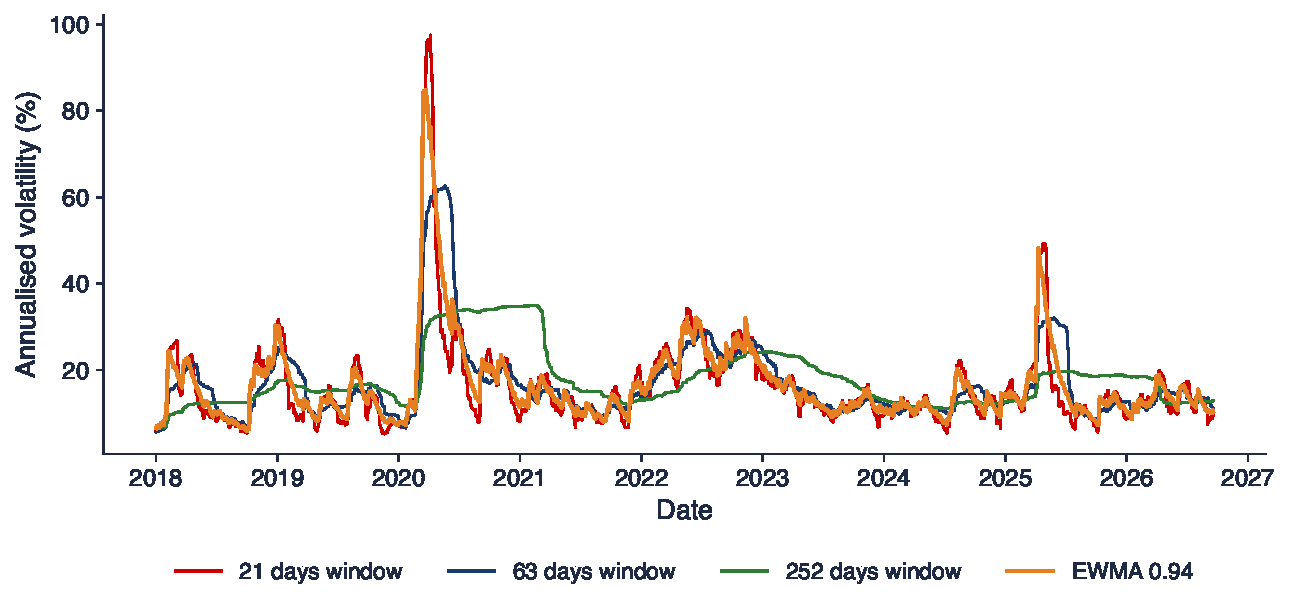
\includegraphics[width=0.96\textwidth,height=0.34\textheight,keepaspectratio]{ch8_sem_b1.pdf}
\end{center}
\vspace{-2mm}
\begin{itemize}
    \item $a = 252$; întregul eșantion 18{,}0\%; pe 18 septembrie 2026: 21 de zile 9{,}6\%, 63 de zile 11{,}1\%, 252 de zile 12{,}9\%, EWMA 10{,}4\%
    \item Maximele din 2020: 97{,}5\% (6 aprilie 2020), 62{,}6\% (20 mai 2020), 34{,}7\% (28 decembrie 2020), EWMA 84{,}8\% (24 martie 2020)
    \item Pe 15 iunie 2020, volatilitatea pe 63 de zile a scăzut de la 50{,}4\% la 43{,}0\% (ziua crahului din 16 martie a ieșit din fereastră); EWMA a trecut de la 35{,}6\% la 34{,}6\%
    \item Interpretare: EWMA; scăderea estimării pe 63 de zile este efectul de fantomă, nu o știre; valoarea pe 252 de zile reflectă încă luna martie
\end{itemize}\sfmquantlet{Ch_08}{SFM_ch8_seminar}
\end{frame}

\begin{frame}{B2: BET și Bitcoin [Propus]}
\itemsize{\footnotesize}
\begin{itemize}
\item \textbf{Întrebarea}: cît de volatile sînt BET și Bitcoin în comparație cu S\&P 500, azi și la sfîrșitul lui 2017? Model: B1.
\item \textbf{Date}: BET din 1997, Bitcoin din 2014, S\&P 500 din 1990, randamente logaritmice zilnice în \%
\item \textbf{Cerințe}
\begin{enumerate}
    \item Calculați numărul de observații pe an și volatilitatea anuală pe întregul eșantion pentru fiecare serie.
    \item Anualizați Bitcoin și cu 252 și dați eroarea în \%.
    \item Raportați volatilitatea pe 252 de zile la sfîrșitul lui 2017 și la sfîrșitul eșantionului, precum și maximul volatilității pe 63 de zile, cu anul lui.
    \item Interpretare: a devenit Bitcoin un activ cu o volatilitate asemănătoare acțiunilor?
\end{enumerate}
\item \textbf{Raportați}: un tabel și două fraze
\item Notebook: secțiunea B2
\end{itemize}
\end{frame}

\ifsolutions
\begin{frame}{B2: rezolvare [Propus]}
\itemsize{\footnotesize}
\begin{center}
\footnotesize
\begin{tabular}{lrrrrrr}
\toprule
& $a$ & \textbf{Vol. anuală} & \textbf{252 de zile, 2017} & \textbf{252 de zile, final} & \textbf{Max. 63 de zile} & \textbf{Anul} \\
\midrule
S\&P 500 & 252 & 18{,}0\% & 6{,}7\% & 12{,}9\% & 72{,}5\% & 2008 \\
BET & 250 & 23{,}4\% & 10{,}4\% & 16{,}0\% & 66{,}6\% & 2009 \\
Bitcoin & 365 & 66{,}6\% & 101{,}3\% & 47{,}2\% & 154{,}8\% & 2018 \\
\bottomrule
\end{tabular}
\end{center}
\begin{itemize}
    \item Bitcoin cu $\sqrt{252}$: 55{,}3\% în loc de 66{,}6\%: valoarea corectă este cu 20{,}4\% mai mare
    \item Interpretare: nu; volatilitatea Bitcoin pe 252 de zile a scăzut de la 101{,}3\% (sfîrșitul lui 2017) la 47{,}2\%, încă de 3{,}7 ori mai mare decît cea a S\&P 500 și de 3{,}0 ori mai mare decît cea a BET
\end{itemize}\sfmquantlet{Ch_08}{SFM_ch8_seminar}
\end{frame}
\fi

\begin{frame}{B3: estimatori de amplitudine pentru S\&P 500 [Rezolvat]}
\itemsize{\footnotesize}
\begin{itemize}
\item \textbf{Întrebarea}: dau estimatorii de amplitudine aceeași volatilitate ca prețurile de închidere pentru S\&P 500?
\item \textbf{Date}: OHLC S\&P 500 din 2008 ($T = 4\,707$ de zile)
\item \textbf{Cerințe}
\begin{enumerate}
    \item Calculați $o_t$, $u_t$, $d_t$, $c_t$ și cei cinci estimatori pe întregul eșantion, anualizați.
    \item Descompuneți $\mathrm{Var}(r_t) = \mathrm{Var}(o_t) + \mathrm{Var}(c_t) + 2\,\mathrm{Cov}(o_t, c_t)$.
    \item Desenați estimările pe ferestre mobile de 21 de zile din 2025.
    \item Interpretare: de ce sînt Parkinson, Garman--Klass și Rogers--Satchell sub estimatorul închidere--închidere?
\end{enumerate}
\item \textbf{Raportați}: graficul, cinci volatilități, o descompunere și două fraze
\item Notebook: secțiunea B3
\end{itemize}
\end{frame}

\begin{frame}{B3: rezolvare [Rezolvat]}
\itemsize{\scriptsize}
\begin{center}
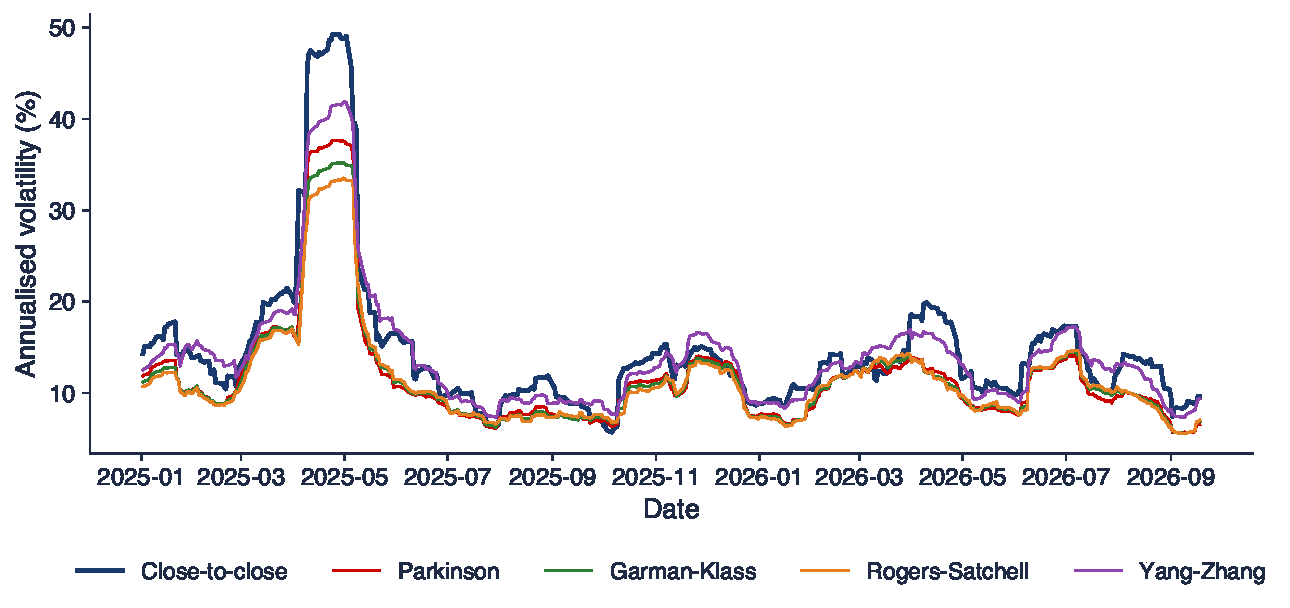
\includegraphics[width=0.96\textwidth,height=0.34\textheight,keepaspectratio]{ch8_sem_b3.pdf}
\end{center}
\vspace{-2mm}
\begin{itemize}
    \item Volatilitatea anuală: CC 19{,}9\%, Parkinson 15{,}4\%, GK 14{,}6\%, RS 14{,}4\%, YZ 16{,}3\%
    \item Varianțe zilnice (\%$^2$): $1{,}568 = 0{,}176 + 1{,}194 + 0{,}197$; noaptea reprezintă 13\% din $\mathrm{Var}(o) + \mathrm{Var}(c)$; $\mathrm{corr}(o, c) = 0{,}22$
    \item Interpretare: acești estimatori văd doar ședința de tranzacționare, deci ratează varianța overnight și termenul de covarianță; YZ adaugă noaptea, dar nu și covarianța
\end{itemize}\sfmquantlet{Ch_08}{SFM_ch8_seminar}
\end{frame}

\begin{frame}{B4: DAX, Bitcoin și TLV [Propus]}
\itemsize{\footnotesize}
\begin{itemize}
\item \textbf{Întrebarea}: pentru care dintre DAX, Bitcoin și Banca Transilvania sînt estimatorii de amplitudine apropiați de estimatorul închidere--închidere? Model: B3.
\item \textbf{Date}: OHLC DAX din 2006, Bitcoin din 2014, OHLC ajustat TLV din 2010
\item \textbf{Cerințe}
\begin{enumerate}
    \item Calculați cei cinci estimatori anualizați pentru fiecare activ.
    \item Calculați ponderea nopții și $\mathrm{corr}(o_t, c_t)$.
    \item Ordonați activele după raportul Parkinson / CC.
    \item Interpretare: pentru ce activ ați putea înlocui estimatorul închidere--închidere cu Parkinson?
\end{enumerate}
\item \textbf{Raportați}: un tabel și două fraze
\item Notebook: secțiunea B4
\end{itemize}
\end{frame}

\ifsolutions
\begin{frame}{B4: rezolvare [Propus]}
\itemsize{\footnotesize}
\begin{center}
\footnotesize
\begin{tabular}{lrrrrrrr}
\toprule
& CC & P & GK & RS & YZ & \textbf{Ponderea nopții} & $\mathrm{corr}(o, c)$ \\
\midrule
DAX & 20{,}9 & 16{,}7 & 16{,}6 & 16{,}6 & 20{,}3 & 31\% & ${0{,}02}$ \\
Bitcoin & 66{,}6 & 63{,}5 & 62{,}4 & 62{,}5 & 63{,}2 & 0\% & ${0{,}02}$ \\
TLV & 26{,}6 & 21{,}5 & 20{,}6 & 21{,}0 & 25{,}6 & 26\% & ${-0{,}08}$ \\
\bottomrule
\end{tabular}
\end{center}
\begin{itemize}
    \item Bitcoin: fără noapte (piață deschisă 24 de ore), toți estimatorii diferă de CC cu cel mult cîteva puncte procentuale
    \item DAX și TLV: o pondere mare a nopții; Parkinson, GK și RS mult sub CC, YZ apropiat de CC
    \item Interpretare: Bitcoin; pentru piețele care se închid noaptea folosiți Yang--Zhang, niciodată doar Parkinson
\end{itemize}\sfmquantlet{Ch_08}{SFM_ch8_seminar}
\end{frame}
\fi

\begin{frame}{B5: volatility clustering la S\&P 500 [Rezolvat]}
\itemsize{\footnotesize}
\begin{itemize}
\item \textbf{Întrebarea}: sînt mărimea și semnul randamentelor S\&P 500 la fel de previzibile?
\item \textbf{Date}: închiderile S\&P 500 din 1990, randamente logaritmice zilnice în \%
\item \textbf{Cerințe}
\begin{enumerate}
    \item Desenați ACF-ul lui $r_t$, $r_t^2$ și $|r_t|$ pentru decalajele 1--50, cu banda de 95\% pentru date i.i.d.
    \item Raportați $\hat\rho_1, \dots, \hat\rho_5$ pentru $r_t$ și pentru $r_t^2$.
    \item Calculați statistica Ljung--Box $Q(10)$ pentru $r_t$, $r_t^2$ și $|r_t|$, precum și statistica ARCH-LM(5) cu $R^2$-ul ei.
    \item Interpretare: contrazice volatility clustering eficiența pieței în formă slabă?
\end{enumerate}
\item \textbf{Raportați}: graficul, zece autocorelații, patru statistici și două fraze
\item Notebook: secțiunea B5
\end{itemize}
\end{frame}

\begin{frame}{B5: rezolvare [Rezolvat]}
\itemsize{\scriptsize}
\begin{center}
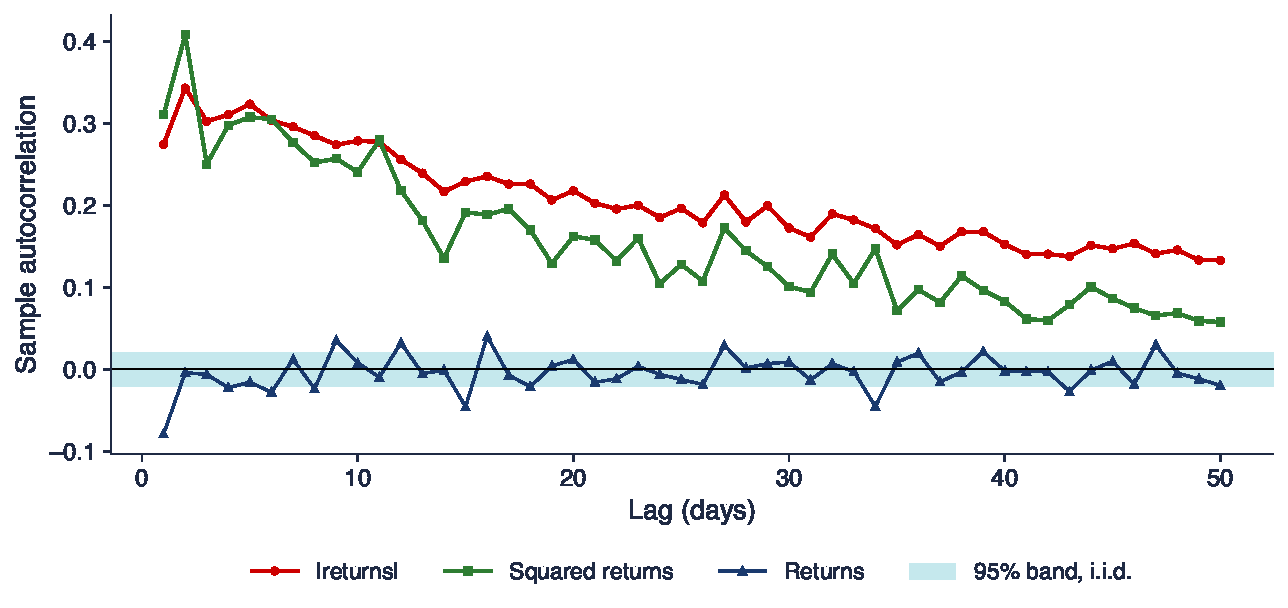
\includegraphics[width=0.96\textwidth,height=0.34\textheight,keepaspectratio]{ch8_sem_b5.pdf}
\end{center}
\vspace{-2mm}
\begin{itemize}
    \item $\hat\rho_{1..5}(r)$: $-0{,}079$; $-0{,}004$; $-0{,}006$; $-0{,}022$; $-0{,}016$; $\hat\rho_{1..5}(r^2)$: $0{,}311$; $0{,}408$; $0{,}250$; $0{,}298$; $0{,}308$; $T = 9\,240$
    \item $Q(10)$: $r$ 90{,}8 (p $<$\,0{,}001), $r^2$ 8\,015, $|r|$ 8\,323 (valoarea critică 18{,}31); ARCH-LM(5) $= 9\,235 \times 0{,}241 = 2\,227$ (valoarea critică 11{,}07)
    \item Interpretare: nu; mărimea este previzibilă, semnul aproape deloc; eficiența privește randamentele previzibile, nu riscul previzibil (\sfmchlink{https://danpele.github.io/SFM/RO/Cursuri/capitol7_piete_eficiente_mers_aleator_vr.pdf}{Capitolul 7})
\end{itemize}\sfmquantlet{Ch_08}{SFM_ch8_seminar}
\end{frame}

\begin{frame}{B6: încă patru serii [Propus]}
\itemsize{\footnotesize}
\begin{itemize}
\item \textbf{Întrebarea}: depinde volatility clustering de la BET, Bitcoin, Banca Transilvania și OMV Petrom de ordinea zilelor? Model: B5.
\item \textbf{Date}: BET din 1997, Bitcoin din 2014, TLV și SNP din 2010
\item \textbf{Cerințe}
\begin{enumerate}
    \item Calculați $\hat\rho_1(r^2)$, $Q(10)$ pentru $r_t^2$, ARCH-LM(5) și excesul de boltire pentru fiecare serie.
    \item Amestecați aleator randamentele (seed 2026) și calculați din nou $Q(10)$ pentru $r_t^2$ și ARCH-LM(5).
    \item Interpretare: de ce amestecarea elimină volatility clustering, dar nu și cozile groase?
\end{enumerate}
\item \textbf{Raportați}: un tabel și două fraze
\item Notebook: secțiunea B6
\end{itemize}
\end{frame}

\ifsolutions
\begin{frame}{B6: rezolvare [Propus]}
\itemsize{\footnotesize}
\begin{center}
\footnotesize
\begin{tabular}{lrrrrrrr}
\toprule
& $T$ & $\hat\rho_1(r^2)$ & $Q(10)$ & ARCH-LM & \textbf{Exc.\ boltire} & $Q(10)$, \textbf{amestecat} (p) & \textbf{LM, amestecat} \\
\midrule
BET & 7\,243 & $0{,}333$ & 2\,500 & 1\,057 & 9{,}9 & 9{,}2 (0{,}511) & 5{,}4 \\
Bitcoin & 4\,384 & $0{,}137$ & 213 & 115 & 12{,}0 & 2{,}0 (0{,}996) & 0{,}5 \\
TLV & 3\,788 & $0{,}122$ & 481 & 253 & 13{,}5 & 2{,}2 (0{,}994) & 1{,}5 \\
SNP & 3\,815 & $0{,}195$ & 505 & 234 & 8{,}9 & 7{,}2 (0{,}703) & 6{,}7 \\
\bottomrule
\end{tabular}
\end{center}
\begin{itemize}
    \item Toate testele resping puternic pentru cele patru serii în ordinea reală; după amestecare niciun test nu respinge
    \item Interpretare: volatility clustering este o proprietate a ordinii zilelor, iar boltirea depinde doar de valori, pe care amestecarea le păstrează
\end{itemize}\sfmquantlet{Ch_08}{SFM_ch8_seminar}
\end{frame}
\fi

\begin{frame}{B7: care prognoză este cea mai bună? [Rezolvat]}
\itemsize{\footnotesize}
\begin{itemize}
\item \textbf{Întrebarea}: ce prognoză simplă a varianței de mîine a S\&P 500 are cea mai mică pierdere din 2010?
\item \textbf{Date}: randamentele S\&P 500 din 1990, închiderile VIX; prognoze pentru 4\,202 de zile din 2010
\item \textbf{Cerințe}
\begin{enumerate}
    \item Construiți prognoze pentru ziua următoare: mediile mobile ale lui $r_t^2$ pe 21, 63 și 252 de zile, EWMA cu $\lambda = 0{,}94$ și $0{,}97$ și $\mathrm{VIX}^2/a$.
    \item Calculați MSE și QLIKE cu variabila proxy $r_t^2$.
    \item Aplicați testul Diebold--Mariano pentru EWMA 0,94 față de fereastra de 21 de zile și pentru VIX față de EWMA 0,94.
    \item Desenați QLIKE pentru EWMA, cu $\lambda$ între 0,80 și 0,995.
    \item Interpretare: este VIX o prognoză mai bună a varianței de mîine decît EWMA?
\end{enumerate}
\item \textbf{Raportați}: un tabel cu douăsprezece valori, două teste, graficul și două fraze
\item Notebook: secțiunea B7
\end{itemize}
\end{frame}

\begin{frame}{B7: rezolvare [Rezolvat]}
\itemsize{\scriptsize}
\begin{center}
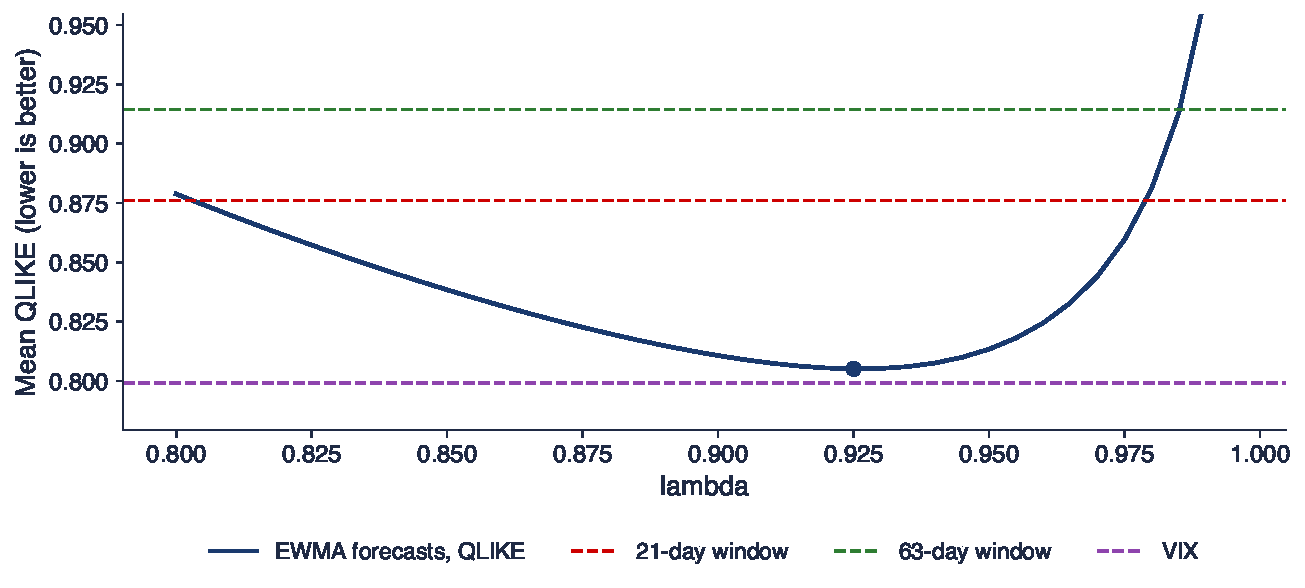
\includegraphics[width=0.96\textwidth,height=0.30\textheight,keepaspectratio]{ch8_sem_b7.pdf}
\end{center}
\vspace{-2mm}
\begin{center}
\scriptsize
\begin{tabular}{lrrrrrr}
\toprule
& 21 & 63 & 252 & EWMA 0,94 & EWMA 0,97 & VIX \\
\midrule
MSE & 18{,}99 & 20{,}77 & 21{,}43 & 17{,}77 & 19{,}02 & 16{,}70 \\
QLIKE & 0{,}876 & 0{,}914 & 1{,}099 & 0{,}808 & 0{,}844 & 0{,}799 \\
\bottomrule
\end{tabular}
\end{center}
\begin{itemize}
    \item DM: EWMA 0,94 față de 21 de zile $t = -4{,}50$ (p $<$\,0{,}001); VIX față de EWMA 0,94 $t = -0{,}32$ (p = 0{,}751); cel mai bun $\lambda = 0{,}925$
    \item Interpretare: nu; VIX are pierderi puțin mai mici, dar diferența nu este semnificativă; ambele sînt mai bune decît ferestrele mobile
\end{itemize}\sfmquantlet{Ch_08}{SFM_ch8_seminar}
\end{frame}

\begin{frame}{B8: cel mai bun $\lambda$ pentru BET și Bitcoin [Propus]}
\itemsize{\footnotesize}
\begin{itemize}
\item \textbf{Întrebarea}: este $\lambda = 0{,}94$ din RiskMetrics o alegere bună pentru BET și pentru Bitcoin? Model: B7.
\item \textbf{Date}: BET din 1997 și Bitcoin din 2014; prognoze din 2010 (BET) și din 2016 (Bitcoin)
\item \textbf{Cerințe}
\begin{enumerate}
    \item Calculați QLIKE pentru prognozele EWMA ale zilei următoare, cu $\lambda$ între 0,80 și 0,995, și găsiți cel mai bun $\lambda$.
    \item Raportați QLIKE pentru cel mai bun $\lambda$, pentru 0,94 și pentru 0,97, precum și timpul de înjumătățire al celui mai bun $\lambda$.
    \item Aplicați testul Diebold--Mariano pentru cel mai bun $\lambda$ față de 0,94.
    \item Interpretare: ați folosi $\lambda = 0{,}94$ pentru ambele serii?
\end{enumerate}
\item \textbf{Raportați}: un tabel și două fraze
\item Notebook: secțiunea B8
\end{itemize}
\end{frame}

\ifsolutions
\begin{frame}{B8: rezolvare [Propus]}
\itemsize{\footnotesize}
\begin{center}
\footnotesize
\begin{tabular}{lrrrrrr}
\toprule
& \textbf{Cel mai bun} $\lambda$ & \textbf{Timp de înjumătățire} & QLIKE, \textbf{optim} & QLIKE, 0,94 & QLIKE, 0,97 & DM $t$ (p) \\
\midrule
BET & 0{,}885 & 5{,}7 & 0{,}851 & 0{,}872 & 0{,}923 & ${-1{,}89}$ (0{,}059) \\
Bitcoin & 0{,}970 & 22{,}8 & 3{,}388 & 3{,}408 & 3{,}388 & ${-0{,}76}$ (0{,}449) \\
\bottomrule
\end{tabular}
\end{center}
\begin{itemize}
    \item BET: cel mai bun este un EWMA mai rapid; cîștigul față de 0,94 este la limită (p = 0{,}059); Bitcoin: cel mai bun este un EWMA mai lent, dar nu semnificativ mai bun decît 0,94
    \item Interpretare: da, ca regulă simplă comună; pierderile din jurul optimului variază puțin, iar un singur $\lambda$ pentru toate activele este mai ușor de justificat
\end{itemize}\sfmquantlet{Ch_08}{SFM_ch8_seminar}
\end{frame}
\fi


%=============================================================================
\section{Partea C: întrebări deschise și critica unui răspuns AI}
%=============================================================================

\begin{frame}{C1: ce estimator pentru acțiunile BVB? [Propus]}
\itemsize{\footnotesize}
\begin{itemize}
\item \textbf{Întrebarea}: îmbunătățesc estimatorii de amplitudine prognozele de volatilitate pentru acțiunile puțin lichide de la Bursa de Valori București?
\item \textbf{Date}: OHLC ajustat pentru TLV, SNP, BRD și TGN din 2010; S\&P 500 din 2008 ca termen de comparație; modele: B3, B7
\item \textbf{Cerințe}
\begin{enumerate}
    \item Calculați ponderea zilelor de tranzacționare cu închiderea neschimbată, precum și rapoartele Parkinson / CC și YZ / CC ale volatilității pe întregul eșantion.
    \item Calculați QLIKE (proxy $r_t^2$) pentru prognozele zilei următoare date de varianțele CC, Parkinson și YZ pe 21 de zile, din 2010.
    \item Comparați cele patru acțiuni cu S\&P 500.
    \item Enumerați două motive pentru care cel mai bun estimator poate diferi de la o acțiune la alta.
    \item Interpretare: de ce date ați avea nevoie pentru a explica diferențele?
\end{enumerate}
\item \textbf{Raportați}: un tabel și un plan de proiect
\item Notebook: secțiunea C1
\end{itemize}
\end{frame}

\ifsolutions
\begin{frame}{C1: analiză de referință [Propus]}
\itemsize{\footnotesize}
\begin{center}
\footnotesize
\begin{tabular}{lrrrrrr}
\toprule
& \textbf{Închidere neschimbată} & P/CC & YZ/CC & QLIKE CC & QLIKE P & QLIKE YZ \\
\midrule
TLV & 8{,}7\% & 0{,}81 & 0{,}96 & 2{,}022 & 2{,}185 & 2{,}039 \\
SNP & 7{,}9\% & 0{,}87 & 1{,}05 & 1{,}866 & 1{,}864 & 1{,}791 \\
BRD & 9{,}7\% & 0{,}90 & 1{,}10 & 1{,}905 & 1{,}940 & 1{,}872 \\
TGN & 10{,}3\% & 0{,}87 & 1{,}04 & 1{,}750 & 1{,}744 & 1{,}636 \\
S\&P 500 & 0{,}0\% & 0{,}78 & 0{,}82 & 0{,}880 & 1{,}009 & 0{,}890 \\
\bottomrule
\end{tabular}
\end{center}
\begin{itemize}
    \item YZ dă cel mai mic QLIKE pentru SNP, BRD și TGN; CC este cel mai bun pentru TLV și pentru S\&P 500; Parkinson singur nu este niciodată clar cel mai bun
    \item Motive: ponderea nopții, tranzacționarea discretă care micșorează amplitudinea, licitația de deschidere, deschideri cu prețuri vechi; diferențele cer teste DM înainte de orice concluzie
    \item Date pentru un proiect: tranzacțiile sau volumele intrazilnice, numărul de tranzacții pe zi, free float-ul fiecărei acțiuni
\end{itemize}\sfmquantlet{Ch_08}{SFM_ch8_seminar}
\end{frame}
\fi

\begin{frame}{C2: verificați un răspuns AI [Propus]}
\itemsize{\scriptsize}
\begin{itemize}
    \item Un student a cerut unui asistent AI să rezume volatilitatea S\&P 500 și a Bitcoin. Răspunsul:
    \item \aiprompt{(a) Din 2008 volatilitatea Parkinson a S\&P 500 este 15{,}4\%, iar cea închidere--închidere 19{,}9\%; Parkinson este de circa cinci ori mai eficient, deci volatilitatea reală este 15{,}4\%.}
    \item \aiprompt{(b) Statistica Ljung-Box Q(10) a randamentelor S\&P 500 este 90{,}8 (p < 0,001), deci S\&P 500 prezintă volatility clustering.}
    \item \aiprompt{(c) EWMA cu lambda = 0,94 are un timp de înjumătățire de circa 94 de zile.}
    \item \aiprompt{(d) Abaterea standard zilnică a Bitcoin este 3{,}49\%, deci volatilitatea anuală este 3{,}49 x sqrt(252) = 55{,}3\%.}
    \item \aiprompt{(e) Din 1990, VIX a fost peste volatilitatea realizată din următoarele 21 de zile în circa 86\% din zile.}
    \item Cerințe
    \begin{itemize}
        \item 1. Pentru fiecare afirmație, precizați dacă este corectă; dacă nu este, formulați afirmația corectă și, acolo unde se poate, dați valoarea corectă din notebook (secțiunea C2).
        \item 2. Raportați: o listă de cinci verdicte, fiecare cu un rînd de justificare.
    \end{itemize}
\end{itemize}
\end{frame}

\ifsolutions
\begin{frame}{C2: rezolvare [Propus]}
\itemsize{\footnotesize}
\begin{itemize}
    \item (a) Greșit: eficiența privește varianța estimatorului, nu deplasarea; Parkinson ratează noaptea (13\% din varianță) și covarianța dintre noapte și zi ($\mathrm{corr} = 0{,}22$); YZ dă 16{,}3\%
    \item (b) Greșit: $Q(10)$ pe randamente testează autocorelația mediei; volatility clustering se testează pe $r_t^2$: $Q(10) = 8\,015$
    \item (c) Greșit: $\ln 0{,}5/\ln 0{,}94 = 11{,}2$ zile
    \item (d) Greșit: Bitcoin se tranzacționează 365 de zile pe an: $3{,}49 \times \sqrt{365} = 66{,}6\%$
    \item (e) Corect: prima de risc a varianței face ca volatilitatea implicită să fie de obicei mai mare decît cea realizată
\end{itemize}\sfmquantlet{Ch_08}{SFM_ch8_seminar}
\end{frame}
\fi


%=============================================================================
\section{Încheiere}
%=============================================================================

\begin{frame}{Idei de reținut}
\itemsize{\small}
\begin{itemize}
    \item Anualizați cu frecvența reală: 252 pentru piețele de acțiuni, 365 pentru Bitcoin
    \item Ferestrele scurte reacționează repede, cele lungi netezesc estimarea; EWMA reacționează fără efect de fantomă
    \item Estimatorii de amplitudine sînt preciși, dar văd doar ședința: folosiți Yang--Zhang cînd piața se închide noaptea
    \item Volatility clustering se testează pe $r_t^2$ (Ljung--Box, ARCH-LM), nu pe $r_t$
    \item Comparați prognozele cu QLIKE și testați diferența; un răspuns AI este o ciornă de verificat
\end{itemize}
\end{frame}

\begin{frame}{După seminar}
\itemsize{\small}
\begin{itemize}
    \item Cursul 8 dezvoltă fiecare temă de azi: volatilitatea istorică și EWMA, volatilitatea de amplitudine și cea realizată, volatility clustering, VIX, evaluarea prognozelor
    \item Încercați cerințele [Propus] în notebook; rezolvările se discută la seminar
    \item C1 poate deveni un proiect de echipă: toate acțiunile din BET, grupe de lichiditate, teste Diebold--Mariano
    \item Lectură: \refFHH, cap.~13; exerciții în \refBHL, cap.~13; \refTsay, cap.~3.1
\end{itemize}
\end{frame}


%=============================================================================
\section{Bibliografie}
%=============================================================================

\begin{frame}{Bibliografie}
\itemsize{\tiny}
\begin{itemize}
    \item Borak, S., Härdle, W.K., López-Cabrera, B. (2013). \href{https://doi.org/10.1007/978-3-642-33929-5}{\textit{Statistics of Financial Markets: Exercises and Solutions}}, 2nd ed. Springer.
    \item Cboe Global Markets (2026). \href{https://www.cboe.com/tradable_products/vix/}{Cboe Volatility Index (VIX)}. Product page and methodology.
    \item Diebold, F.X., Mariano, R.S. (1995). \href{https://doi.org/10.1080/07350015.1995.10524599}{Comparing predictive accuracy}. \textit{Journal of Business \& Economic Statistics}, 13(3), 253--263.
    \item Engle, R.F. (1982). \href{https://doi.org/10.2307/1912773}{Autoregressive conditional heteroscedasticity with estimates of the variance of United Kingdom inflation}. \textit{Econometrica}, 50(4), 987--1007.
    \item Franke, J., Härdle, W.K., Hafner, C.M. (2019). \href{https://doi.org/10.1007/978-3-030-13751-9}{\textit{Statistics of Financial Markets: An Introduction}}, 5th ed. Springer.
    \item Garman, M.B., Klass, M.J. (1980). \href{https://doi.org/10.1086/296072}{On the estimation of security price volatilities from historical data}. \textit{Journal of Business}, 53(1), 67--78.
    \item J.P. Morgan/Reuters (1996). \href{https://www.msci.com/documents/10199/5915b101-4206-4ba0-aee2-3449d5c7e95a}{\textit{RiskMetrics -- Technical Document}}, 4th ed. New York: Morgan Guaranty Trust Company.
    \item Ljung, G.M., Box, G.E.P. (1978). \href{https://doi.org/10.1093/biomet/65.2.297}{On a measure of lack of fit in time series models}. \textit{Biometrika}, 65(2), 297--303.
    \item McLeod, A.I., Li, W.K. (1983). \href{https://doi.org/10.1111/j.1467-9892.1983.tb00373.x}{Diagnostic checking ARMA time series models using squared-residual autocorrelations}. \textit{Journal of Time Series Analysis}, 4(4), 269--273.
    \item Parkinson, M. (1980). \href{https://doi.org/10.1086/296071}{The extreme value method for estimating the variance of the rate of return}. \textit{Journal of Business}, 53(1), 61--65.
    \item Patton, A.J. (2011). \href{https://doi.org/10.1016/j.jeconom.2010.03.034}{Volatility forecast comparison using imperfect volatility proxies}. \textit{Journal of Econometrics}, 160(1), 246--256.
    \item Rogers, L.C.G., Satchell, S.E. (1991). \href{https://doi.org/10.1214/aoap/1177005835}{Estimating variance from high, low and closing prices}. \textit{Annals of Applied Probability}, 1(4), 504--512.
    \item Tsay, R.S. (2010). \href{https://doi.org/10.1002/9780470644560}{\textit{Analysis of Financial Time Series}}, 3rd ed. Wiley.
    \item Yang, D., Zhang, Q. (2000). \href{https://doi.org/10.1086/209650}{Drift-independent volatility estimation based on high, low, open, and close prices}. \textit{Journal of Business}, 73(3), 477--492.
\end{itemize}
\end{frame}

\end{document}
